% !TeX root = ../../main.tex

\chapter{Distributed Job Dispatching in Edge Computing Networks with Random Transmission Latency: A Low-Complexity POMDP Approach}
\label{ch3}

In the previous chapter, we have investigated the centralized job dispatching problem in edge computing networks with random job arrivals, uploading latency and computation time.
In this Chapter, we extend the problem to a distributed job dispatching problem in edge computing networks with random signaling latency among edge servers.
The edge servers are deployed in closer proximity to mobile IoT devices than the traditional cloud computing infrastructure, which enable computation offloading from mobile IoT devices (e.g., mobile phones, video surveillance cameras, etc.) via Access Points (APs) and alleviate the communication overhead.
This brings new challenges to online job dispatching algorithm design, where the importance of cooperation among edge servers with outdated and partial signaling information is addressed.

%NOTE: (1b) why multiple edge servers deployed
Since the edge servers are usually with limited computation resources, the distributed deployment of edge computing servers in the network is favored.
Therefore, a fundamental problem in edge computing is to investigate the cooperative job dispatching among multiple APs and edge servers as illustrated in \figurename~\ref{fig:system}.
More specifically, mobile IoT devices offload jobs through APs, each of which performs as a job dispatcher to choose edge servers processing the data. Typically, there are a large number of APs in a Metropolitan Area Network (MAN). Some APs are co-located with edge servers while others are not.

\begin{figure*}[htp!]
    \centering
    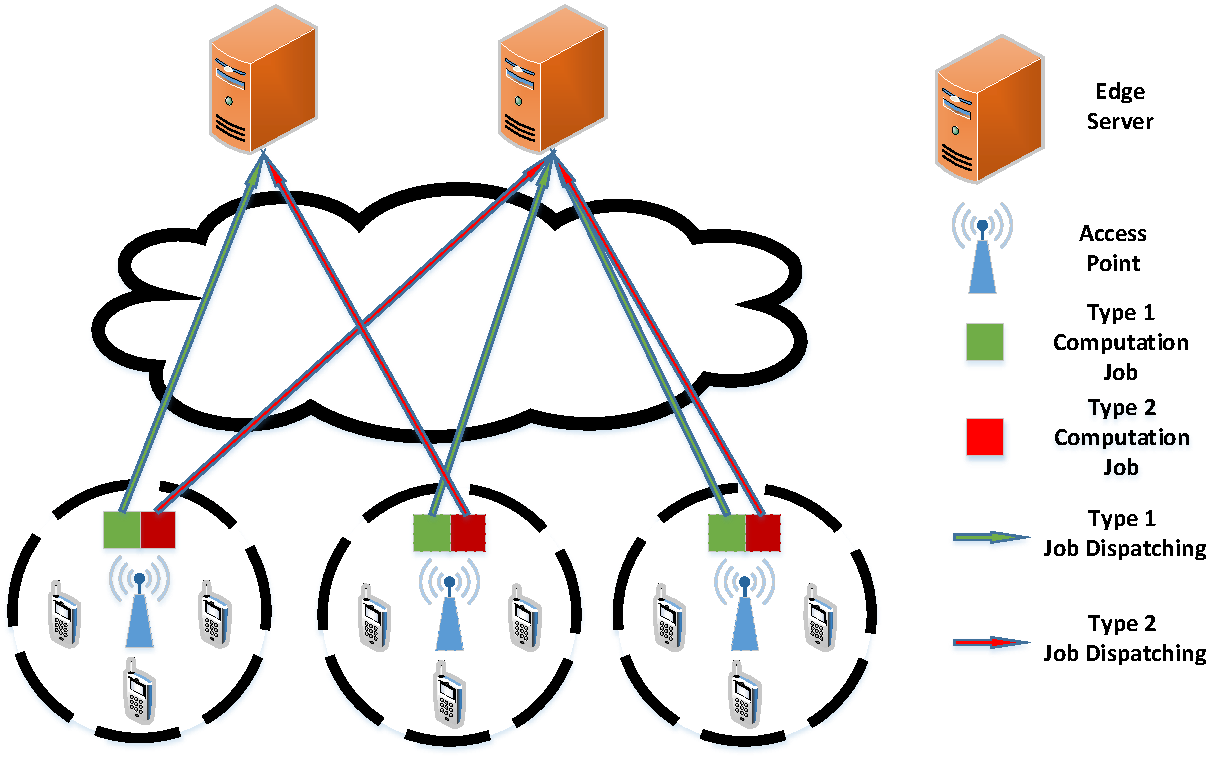
\includegraphics[width=1.0\textwidth]{chapter3/system-model.pdf}
    \caption{The illustration of system model.}
    \label{fig:system}
\end{figure*}

%NOTE: (2) Motivation with MAN and Distributed Dispatchers
%NOTE: (2a) why cooperation is needed; cooperation in MAN is another challenge
Most existing works assume a centralized job dispatcher, which has timely and complete knowledge of the global system status and distributes the dispatching decisions to all the APs without delay \cite{tan-online,IOTJ18-FanQ,mdp-globecom,mdp-tvt,MASS18-MengZ}.
However, the edge computing systems are usually deployed at Metropolitan Area Network (MAN) scale in practice, e.g., the Edge Computing Interconnect (ECI) Network \cite{MAN-ECI}, where the latency of information sharing among APs and edge servers is non-negligible. Moreover, according to the MAN performance analysis in \cite{MAN-LATENCY}, the end-to-end transmission latency is highly variable with respect to different hours of the day and IoT devices' locations in a MAN, which implies the randomness in the job uploading latency from APs to edge servers as well as the signaling latency (i.e., the transmission latency of the {system status} information).
%NOTE: (2b) challenge brought by random latency
There have been several works in the literature considering random transmission latency of job delivery in the edge computing network \cite{latency-EDGE19,MOBIHOC19-ZhouZ,IOTJ18-FanQ,TOC19-LiuC,JSAC19-AlameddineHA}.
However, there are few works considering the random signaling latency of information sharing among distributed dispatchers \cite{tan-online,TWC18-LyuX}.
In fact, it is full of {challenges} to consider random transmission latency in both job uploading and signaling in edge systems.
\begin{itemize}
    % 1) signaling latency: centralized/distributed, outdated information
    \item Firstly, the centralized dispatcher design is discouraged for unpredictable signaling latency, as the distribution of dispatching decisions would consume extra random time. For distributed dispatchers design, the information exchange among distributed dispatchers also suffers from significant signaling overhead and outdated information.
    % 2) uploading latency: inconsistency information exchange;
    \item Secondly, as the job arrivals at edge servers are unknown in advance because of random uploading latency, different dispatchers would have inconsistent system information even if the signaling latency is fixed.
\end{itemize}

To conclude, the random transmission latency may introduce ineliminable estimation errors on the number of jobs at APs or edge servers in the system.

% NOTE: (3) Our contributions
In this chapter, we address the above challenges by leveraging a partially observable Markov decision process (POMDP) problem formulation, and a novel low-complexity approximate MDP solution framework is proposed.
Specifically, we consider a practical scenario where the APs cooperatively upload different types of jobs to different edge servers with random uploading latency, and the APs receive the partial system state information suffering from random signaling latency (i.e., the global system state is always partially available and outdated at the APs).
The major contributions are summarized below.
\begin{itemize}
    \item The distributed and cooperative job dispatching design with outdated and partial information is formulated as a POMDP problem.
    Different from the conventional value or policy iteration of the Bellman's equations where global or historical system states are requested in numerical calculation, a novel low-complexity approximate MDP solution framework via \emph{alternative policy iteration} is proposed, where the dispatching policies of all APs are updated distributedly and alternatively based on the {closed-form expression} of the approximate local value function.
    Thus, the conventional complicated POMDP solution is avoided.
    \item Both analytical performance lower bound and tighter semi-analytical lower bound are derived for the proposed distributed dispatching policy. In the conventional approximate MDP methods, the performance is usually evaluated numerically.
    The lower bounds not only justify the reliability of the proposed policy but also provide a method of quick performance evaluation.
    \item We extend our solution framework {\Dalgname} with an efficient online learning approach to evaluate the approximate value function when the priori knowledge of the system randomness is absent.
    \item We conduct extensive simulations based on the Google Cluster trace, compared with three heuristic benchmarks. The evaluation results show that {\Dalgname} can achieve as high as $20.67\%$ reduction in average job response time and consistently perform well under various parameter settings of signaling latency, job arrival intensity and job processing time. {Moreover, the online learning algorithm converges fast.}
\end{itemize}

The remainder of this chapter is organized as follows.
In Section \ref{sec:chapter3-model}, we elaborate the system model and the signaling mechanism with random transmission latency.
In Section \ref{sec:chapter3-formulation}, we formulate the global-wise optimization of dispatching decisions at all APs as a POMDP.
In Section \ref{sec:chapter3-algorithm}, we propose a novel low-complexity approximate MDP solution framework, called {\Dalgname}.
% where the policy iteration could be applied distributedly on each AP {with partial and outdated information}.
In Section \ref{sec:chapter3-rl-alg}, the solution framework is extended with reinforcement learning technique to handle the unknown statistics.
The numerical analysis of the proposed solution is provided in Section \ref{sec:chapter3-evaluation}, and the conclusion is drawn in Section \ref{sec:chapter3-conclusion}.


%=================================================================================================%
%=================================================================================================%

\section{System Model}
\label{sec:chapter3-model}
In this section, we elaborate the model of edge computing networks with random job arrivals, uploading latency and computation time, as well as the signaling mechanism with periodic broadcast.
%----------------------------------------------------------------------------------------%
\subsection{Network Model}
We consider an edge computing system with $K$ Access Points (APs) and $M$ edge servers, which are connected in an edge network as illustrated in \figurename~\ref{fig:system}.
The sets of APs and edge servers are denoted as $\apSet \define \set{1,\dots,K}$ and $\esSet \define \set{1,\dots,M}$, respectively.
An edge server is typically deployed and collocated with an AP so that mobile devices can upload jobs efficiently.
The communication latency among these APs and edge servers is random.
Each AP collects the computation jobs from the {mobile IoT devices} within its coverage, and makes dispatching {decisions} on the edge servers for each job.
It is assumed that the $k$-th AP only dispatches the computation jobs to the edge servers within a certain number of hops.
Let $\esSet_{k} \subseteq \esSet$ be the subset of edge servers which can compute the jobs from the $k$-th AP, and $\apSet_{m}$ be the subset of APs, which may upload jobs to the $m$-th edge server.
We refer to $\esSet_{k}$ as the \emph{candidate server set} of the $k$-th AP, $\apSet_{m}$ as the \emph{potential AP set} of the $m$-th edge server, and $\rho_{k,m}$ as the collocation indicator (i.e., $\rho_{k,m}=1$ if $k$-th AP and $m$-th edge server collocated, otherwise $\rho_{k,m}=0$) ($\forall k\in\apSet, m\in\esSet$).

Different APs may have different candidate servers according to their locations in the network.
In this edge computing network, APs and edge servers periodically broadcast their state information (the state information is defined in Section \ref{subsec:chapter3-broadcast}), and one AP updates its strategy of job dispatching when receiving the broadcast state information.
We shall optimize the job dispatching strategy distributed at APs with partially observable state information, where both job uploading and state information broadcasting suffer from random transmission latency.

%NOTE: [job space support and arrival process]
Without loss of generality, it is assumed that there are $J$ types of jobs in this system, which are denoted via the set $\jSpace \define \set{1,\dots,J}$.
The time axis of dispatching is organized by time slots.
The arrivals of the type-$j$ jobs at the $k$-th AP ($\forall k\in\apSet,j\in\jSpace$) in different time slots are assumed to be independent and identically distributed (i.i.d.) Bernoulli random variables, and the arrival probability is denoted as $\lambda_{k,j}$.
Let $B_{k,j}(t) \in \set{0,1}$ represent the event of job arrival, where $B_{k,j}(t)=1$ means one type-$j$ job arrives at the $k$-th AP at the $t$-th time slot, and $B_{k,j}(t)=0$ means otherwise.
Hence,
\begin{align}
    \Pr\{ B_{k,j}(t) = 1 \} = \lambda_{k,j}, \forall t,k\in\apSet,j\in\jSpace.
\end{align}

%NOTE: [uploading process]
Each AP immediately dispatches each type of received jobs to one edge server.
As the APs upload jobs over shared edge networks illustrated in \figurename~\ref{fig:system}, the actual uploading time is random due to random traffics initiated from other enabled services.
Moreover, the notification of uploading completion from edge server to AP also consumes random time slots for the same reason, and thus the uploading time is unknown in advance.
Hence, we assume the uploading time of different types of jobs from different APs to edge servers follow independent and discrete distributions.
Let $\mathbb{U}_{k,m,j}(\Xi)$ be the uploading latency (in terms of time slots) distribution of the type-$j$ jobs from the $k$-th AP to the $m$-th edge server with support $\set{1, \dots, \Xi}$ ($\forall k\in\apSet, m\in\esSet, j\in\jSpace$), where $\Xi$ is the maximum possible uploading time for all jobs and the expectation is denoted as $u_{k,m,j}$.
Specifically, the uploading latency is fixed as $0$ if $\rho_{k,m}=1$ for job uploading to the collocated edge server.

%NOTE: [computation process]
For job computation process on edge servers, we adopt the \emph{unrelated machines assumption} as in \cite{tan-online} where the computation time on different edge servers would follow independent distributions.
Specifically, there are $J$ parallel virtual machines (VMs) running on each edge server for processing the $J$ job types, respectively.
It is assumed that the computation time of different job types on different edge servers follows independent memoryless geometric distribution 
\footnote{In this work, we adopt the memoryless geometric distribution to simplify the elaboration of algorithm. In fact, the proposed algorithm can be easily extended to other distributions.}
with different expectations as in \cite{TOWC18-HuangKb}.
Let $\mathbb{G}(1/c_{m,j})$ be the distribution of the computation time slots for the type-$j$ jobs on the $m$-th edge server, where $\mathbb{G}$ denotes the geometric distribution, $c_{m,j}$ is the expectation.
Let $f_{m,j}$ be its probability mass function (PMF), we have
\begin{align}
    f_{m,j}(x) \define (1-\frac{1}{c_{m,j}})^{x-1} \frac{1}{c_{m,j}}, x=1,2,\dots.
\end{align}
For each job type, the uploaded jobs are computed in a First-Come-First-Serve (FCFS) manner, and a processing queue with a maximum job number $L_{max}$ is established for each VM.
The arrival jobs will be discarded when the processing queue is full.

\begin{remark}[Generalization to Edge-Cloud Model]
    The above network model could be generalized into a computing system with both edge servers and cloud center.
    A cloud center could be treated as a special edge server in our model but with stronger computational capability and larger uploading latency and signaling latency to the APs.
\end{remark}

\subsection{Signaling Mechanism with Periodic Broadcast}
\label{subsec:chapter3-broadcast}
In order to facilitate distributed and cooperative dispatching for the APs, {the signaling mechanism with periodic broadcast is introduced.}
We refer to every $t_B$ time slots as a \emph{broadcast interval}.
As illustrated in \figurename~\ref{fig:brd_timeline}, at the beginning of each broadcast interval, the local state information (LSI) of APs and edge servers are broadcast, and each AP updates its dispatching strategy of job dispatching when observing the broadcast LSIs from some APs and edge servers.
As a remark notice that the observable LSI may be outdated due to transmission latency among APs and edge servers.
The LSI at the APs and edge servers, global state information, and observable state information at the APs are defined below, respectively.

%NOTE: State and Broadcast Information for AP
\begin{definition}[LSI of APs]
    Let $R^{(k)}_{m,j}(\xi,t,n) \in \set{0,1}$ be the indicator of the type-$j$ jobs at the $n$-th time slot of the $t$-th interval.
    Its value is $1$ when there is one job being uploaded from the $k$-th AP to the $m$-th server which has been delivered for $\xi$ time slots, and $0$ otherwise.
    Let $\omega_{k,j}(t)$ be the target edge server for the type-$j$ jobs of the $k$-th AP at the very beginning of the $t$-th broadcast interval.
    The LSI of the $k$-th AP at the beginning of the $t$-th broadcast interval is defined as
    \begin{align}
        \mathcal{R}_{k}(t) \define
        \Paren{
            \Brace{\vec{R}^{(k)}_{m,j}(t,0) \Big| \forall m\in\esSet,j\in\jSpace},
            \mathcal{A}_{k}(t)
        },
    \end{align}
    where
    \begin{align}
        \vec{R}^{(k)}_{m,j}(t,0) \define \Paren{
            R^{(k)}_{m,j}(0,t,0), \dots, R^{(k)}_{m,j}(\Xi,t,0)
        },
    \end{align}
    and
    \begin{align}
        \mathcal{A}_{k}(t) &\define \Brace{\omega_{k,j}(t) \Big| \forall j\in\jSpace}
    \end{align}
    are referred as status of the type-$j$ job uploading from the $k$-th AP to the $m$-th edge server, and the dispatching actions for all types of jobs of the $k$-th AP at the beginning of the $t$-th broadcast interval, respectively.
\end{definition}

%NOTE: State and Broadcast Information for Edge Server
\begin{definition}[LSI of Edge Servers]
    Let $Q_{m,j}({t,n})$ be the number of type-$j$ jobs on the $m$-th edge server at the $n$-th time slot of the $t$-th interval ($\forall m\in\esSet, j\in\jSpace$).
    The LSI of the $m$-th edge server at the $t$-th broadcast interval is defined as
    \begin{align}
        \mathcal{Q}_{m}(t) \define \Brace{
            Q_{m,j}(t, 0) \Big| \forall j\in\jSpace
        }.
    \end{align}
\end{definition}

\begin{definition}[Global State Information]
    The global state information (GSI) of the $t$-th broadcast interval is defined as the aggregation of the broadcast LSIs from all the APs and edge servers, i.e.,
    \begin{align}
        \Stat(t) \define
            \Paren{
                \Brace{\mathcal{R}_{k}(t) \Big| \forall k\in\apSet},
                \Brace{\mathcal{Q}_{m}(t) \Big| \forall m\in\esSet}
            }.
    \end{align}
\end{definition}

%NOTE: Conflict of AP set and partial information definition
As the APs and edge servers may reside in different locations of a MAN, the transmission latency of LSI is not negligible.
It might be inefficient {and costly} for one AP to collect the complete GSI before the update of dispatching policy.
For example, the transmission latency of the LSI from the edge servers outside the \emph{candidate server set} $\esSet_{k}$ to the $k$-th AP may be large, and some broadcast information may be discarded by the routers after a certain number of hops.
In this chapter, we shall investigate the distributed dispatching design based on the \emph{observable state information} at each AP.
Specifically, the \emph{conflict AP sets} and the \emph{observable state information} are defined below, respectively.
\begin{definition}[Conflict AP Set]
    The conflict AP set to the $k$-th AP ($\forall k\in\apSet$) consists of the neighboring APs who share any common edge server with the $k$-th AP, i.e.,
    \begin{align}
        \ccSet_{k} \define \bigcup_{m\in\esSet_{k}} \apSet_{m}.
    \end{align}
\end{definition}

\begin{definition}[Observable State Information]
    \label{def:OSI}
    The observable state information (OSI) of the $k$-th AP ($\forall k\in\apSet$) at the $t$-th broadcast interval is defined as the aggregation of LSIs of the APs in {conflict AP set} and the edge servers in {candidate server set} of the $k$-th AP, i.e.,
    \begin{align}
        \Stat_{k}(t) &\define
        \Paren{
            \Brace{\mathcal{R}_{k'}(t) \Big| \forall k'\in\ccSet_{k}},
            \Brace{\mathcal{Q}_{m}(t) \Big| \forall m\in\esSet_{k}}
        }.
    \end{align}
\end{definition}

\begin{figure*}[t]
    \centering
    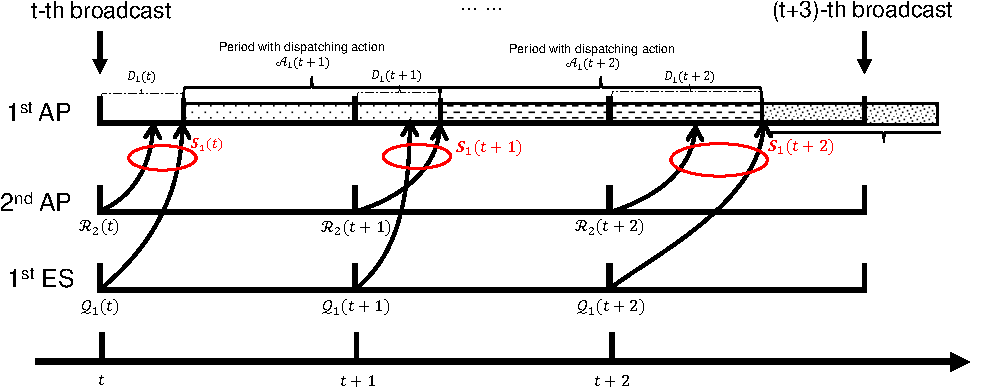
\includegraphics[width=1.0\textwidth]{chapter3/brd-timeline.pdf}
    \caption{The timeline illustration of reception of OSI for the $1$-st AP where $2$-nd AP is in its \emph{conflict AP set} and $1$-st server is in its \emph{candidate server set}.}
    \label{fig:brd_timeline}
\end{figure*}

The $k$-th AP is able to collect its OSI $\Stat_{k}(t)$ at the $\mathcal{D}_{k}(t)$-th time slots of the $t$-th broadcast interval, where the {\emph{\brlatency}} $\mathcal{D}_{k}(t)$ is a random variable.
It is assumed that $\mathcal{D}_{k}(t)$ follows identical and independent distribution in different broadcast interval.
An example is given below to demonstrate how the {\brlatency} affects the reception of OSI and the update of the dispatching strategy.
Moreover, the notations used throughout this chapter are summarized as in Table \ref{table:symbols}.

\begin{example}
    In \figurename~\ref{fig:brd_timeline}, the $2$-nd AP and $1$-st server are in the \emph{conflict AP set} and \emph{candidate server set} of the $1$-st AP, respectively.
    At the beginning of the $t$-th broadcast interval, the dispatching actions $\mathcal{A}_{1}(t)$ is adopted by the $1$-st AP.
    After $\mathcal{D}_{1}(t)$ time slots, it updates the dispatching actions to $\mathcal{A}_{1}(t+1)$ based on its OSI $\Stat_{1}(t)$.
    In the $(t+1)$-th broadcast interval, the $1$-st AP will firstly keep the previous actions $\mathcal{A}_{1}(t+1)$, and then updates the actions $\mathcal{D}_{1}(t+1)$ time slots later based on $\Stat_{1}(t+1)$. The new action is denoted as $\mathcal{A}_{1}(t+2)$.
    The signaling latency $\mathcal{D}_1(t)$ and $\mathcal{D}_1(t+1)$ can be different.
\end{example}

\begin{remark}[Transmission Failure of OSI]
    % [Handling Broadcast Information Transmission Failure]
    % R1-1: How do you deal with the failed transmission of system state information?
    % R2-2: What if the information broadcast by the 2-nd AP is not received by the 1-st AP?
    In the system model, the transmission failure of OSI is tolerable: it can actually be transferred to transmission latency.
    For example, if the $y$-th AP is in the \emph{conflict AP set} of the $k$-th AP and the state information transmission from the $y$-th AP failed, the $k$-th AP may request retransmissions until a successful reception.
    This will raise the transmission latency of OSI, which contributes to the random {\brlatency} $\Delay_{k}(t)$ of the $k$-th AP.
\end{remark}

\begin{table}[htp!]
    \footnotesize
    \centering
    \caption{Table of notations and their descriptions throughout this chapter.}
    \label{table:symbols}
    \begin{tabulary}{1.0\linewidth}{|p{2.5cm}|L|}
        \hline
        Notation                        & Description \\
        \hline
        $\mathcal{K}$                   & The denotation of AP set \\
        $\mathcal{M}$                   & The denotation of edge server set \\
        $\mathcal{K}_{m}$               & The potential AP set of the $m$-th edge server \\
        $\mathcal{M}_{k}$               & The candidate edge server set of the $k$-th AP \\
        $\ccSet_{k}$                    & The conflict AP set of the $k$-th AP  \\
        $\mathcal{J}$                   & The denotation of job types set \\
        $\lambda_{k,j}$                 & The average arrival job rate for the type-$j$ job on the $k$-th AP \\
        $c_{m,j}$                       & The average computation time for the type-$j$ job on the $m$-th edge server \\
        $L_{max}$                       & The maximum job number for each VM \\
        $t_B$                           & The duration of a broadcast interval \\
        $\Xi$                           & The maximum job uploading time \\
        $\xi$                           & The index of time slot of uploading time for one job \\
        $\mathbb{U}_{k,m,j}(\Xi)$       & The uploading latency distribution of the type-$j$ jobs from the $k$-th AP to the $m$-th edge server \\
        $\mathcal{R}_{k}(t)$            & The LSI of the $k$-th AP at the beginning of the $t$-th broadcast interval \\
        $\mathcal{Q}_{m}(t)$            & The LSI of the $m$-th edge server at the beginning of the $t$-th broadcast interval \\
        $D_{k}(t)$                      & The {\brlatency} for the $k$-th AP at the $t$-th broadcast interval \\
        $\mathbb{D}(t)$                 & The vector of all {\brlatency} at the $t$-th broadcast interval \\
        $\Stat(t)$                      & The GSI at the $t$-th broadcast interval \\
        $\Stat_{k}(t)$                  & The OSI of the $k$-th AP at the $t$-th broadcast interval \\
        $\omega_{k,j}(t)$               & The dispatching action for type-$j$ job on the $k$-th AP at the beginning of $t$-th broadcast interval \\
        $\mathcal{A}_{k}(t)$               & The dispatching actions of the $k$-th AP at the beginning of $t$-th broadcast interval \\
        $\Policy(\Stat(t),\Delay(t))$   & The aggregation of individual policy all APs \\
        $\Baseline(\Stat(t),\Delay(t))$ & The proposed baseline policy \\
        $\gamma$                        & The discount factor \\
        $\beta$                         & The weight of overflow penalty \\
        $\mathcal{Y}_{n}$               & The $n$-th subset partition in which the APs update their dispatching actions parallel \\
        $\tilde{\mathcal{A}}(t)$        & The aggregation of dispatching actions of the APs in the subset $\mathcal{Y}_{n}$, where $n \define t \pmod{N}$  \\
        $\hat{\mathcal{A}}(t)$          & The aggregation of dispatching actions of the APs not in the subset $\mathcal{Y}_{n}$, where $n \define t \pmod{N}$ \\
        \hline
    \end{tabulary}
\end{table}

%=================================================================================================%
%=================================================================================================%

\section{POMDP-based Problem Formulation}
\label{sec:chapter3-formulation}
%----------------------------------------------------------------------------------------%
In this section, we formulate the optimization of job dispatching problem of all APs as a Markov decision process (MDP).
Since each AP updates the job dispatching action according to OSI instead of GSI, the MDP problem is a partially observable MDP (POMDP).
Firstly, we give the definitions of \emph{dispatching policy} and \emph{cost function}, together with the \emph{system state} (i.e., the GSI) defined previously, to complete the MDP problem formulation.

\begin{definition}[Dispatching Policy]
    The individual dispatching policy of the $k$-th AP, denoted as $\Omega_{k}$ ($\forall k \in\apSet$), maps from its OSI $\Stat_{k}$ and its {\brlatency} $\mathcal{D}_{k}$ to the dispatching action for each job type, i.e.,
    \begin{align}
        \Omega_{k} \Paren{ \Stat_{k}(t), \mathcal{D}_{k}(t) }
        &\define \mathcal{A}_{k}(t+1)
        \nonumber\\
        &= \Brace{
            \omega_{k,j}(t+1) \Big| \forall j\in\jSpace
        }.
        \label{def:action}
    \end{align}

    The aggregation of individual policy of all APs is referred to as the system dispatching policy $\Policy$.
    Thus,
    \begin{align}
        \Policy\Paren{ \Stat(t), \Delay(t) } \define \Brace{
            \Omega_{1}(\Stat_{1}(t), \mathcal{D}_{1}(t)), \dots, \Omega_{K}(\Stat_{K}(t),\mathcal{D}_{K}(t))
        },
    \end{align}
    where $\Delay(t) \define \set{ \mathcal{D}_{1}(t), \dots, \mathcal{D}_{K}(t) }$.
\end{definition}

The average job response time and packet drop rate are considered as the system cost.
The job response time counts the number of broadcast intervals from job arrival to the accomplishment of computation, which includes the uploading time from the AP to the edge server, the waiting time in the processing queue and the job processing time on the edge server.
According to the Little's law \cite{Little1961}, the average response time per job, counting the number of broadcast intervals from job arrival to the accomplishment of computation, is proportional to the number of jobs in the system, given the job arrival rates at all the APs.
Hence, we define the cost function per broadcast interval as follows, {given the information contained in periodic broadcast.}

\begin{definition}[Cost Function per Broadcast Interval]
    The cost function of the $t$-th broadcast interval with GSI $\Stat(t)$ is defined as
    \begin{align}
        g\Paren{\Stat(t)} \define
            \sum_{m\in\esSet,j\in\jSpace}
            \Brace{&
                \sum_{k\in\apSet} \Inorm{\vec{R}^{(k)}_{m,j}(t,0)} + Q_{m,j}(t,0)
                + \beta \cdot I[Q_{m,j}(t,0)=L_{max}]
            },
    \end{align}
    where $\Inorm{\vec{x}}$ denotes the $L^1$-norm of the vector $\vec{x}$, $\sum_{k\in\apSet} \Inorm{\vec{R}^{(k)}_{m,j}(t,0)}$ measures the number of type-$j$ jobs being uploaded from the $k$-th AP to the $m$-th edge server, $Q_{m,j}(t,0)$ measures the number of type-$j$ jobs on the $m$-th edge server, and $\beta$ is the weight of overflow penalty.
    The cost function per broadcast interval could be taken as a uniform sampling of cost function per time slot.
\end{definition}

Since the job dispatching in one broadcast interval will affect the GSI of the following broadcast intervals, we should consider the joint minimization of the costs of all the broadcast intervals.
Specifically, we consider the following discounted sum of the costs of all the broadcast intervals as the system objective.
\begin{align}
    &\bar{G}(\Stat(1), \Policy) \define
    \lim_{T \to \infty} \mathbb{E}^{\Policy}_{\set{\Stat(t)|\forall t}, \Delay}
    \Bracket{
        \sum_{t=1}^{T} \gamma^{t-1} g\Paren{\Stat(t)} \Big| \Stat(1)
    },
\end{align}
where $\mathbb{E}^{\Policy}_{\set{\Stat(t)|\forall t}}[\cdot]$ denotes the expectation with respect to all possible system states in the future given scheduling policy $\Policy$, and $\gamma \in (0,1)$ is the discount factor.
Hence, the optimization of job dispatching policy can be formulated as the following minimization problem.
\begin{align}
    \textbf{P1:}~
    \min_{\Policy} \bar{G}(\Stat(1), \Policy).
\end{align}

If the GSI $\Stat(t)$ and {\brlatency} $\Delay(t)$ are known to all the APs, the MDP in problem P1 can be solved via the following Bellman's equations as in \cite{sutton1998}.
\begin{align}
    V\Paren{\Stat(t)} =&g\Paren{\Stat(t)}
        + \gamma\mathbb{E}_{\Delay}\bigg\{
            \min_{\Policy(\Stat(t),\Delay(t))}
            \nonumber\\
            &\sum_{\Stat(t+1)} \Pr \Big\{ 
                \Stat(t+1) \Big| \Stat(t), \Policy(\Stat(t), \Delay(t)) \Big\} \cdot V\Big(\Stat(t+1)\Big)
            \bigg\},
    \label{eqn:sp_0}
\end{align}
where the value function $V(\Stat(t))$ of the optimal policy $\Policy^{*}$ (if GSI and {\brlatency} are known to all the APs) is defined as follows.
\begin{align}
    &V\Paren{\Stat(t)} \define
    \lim_{T\to\infty} 
    \mathbb{E}^{\Policy^*}_{\set{\Stat(t)|\forall t}, \Delay} \Bracket{
        \sum_{t=1}^{T} \gamma^{t-1} g\Big( \Stat(t) \Big) \Big| \Stat(1)
    }.
    \label{eqn:val_f}
\end{align}
Moreover, the optimal dispatching policy $\Omega^{*}$ can be obtained by solving the right-hand-side (RHS) of the above Bellman's equations (\ref{eqn:sp_0}).

However, it is infeasible to solve the above Bellman's equations {and achieve the performance of $\Policy^*$ in our considered distributed dispatching scenario.}
This is because each AP (say the $k$-th AP) only has the knowledge of its own OSI $\Stat_{k}(t)$ and local {\brlatency} $\mathcal{D}_{k}(t)$, but the optimal solution (dispatching actions of all APs) for the RHS of Equation (\ref{eqn:sp_0}) depends on the GSI and the knowledge of global {\brlatency}.
Thus, problem P1 is actually a POMDP, which is further demonstrated by a toy example below.

\begin{figure*}[htp!]
    \centering
    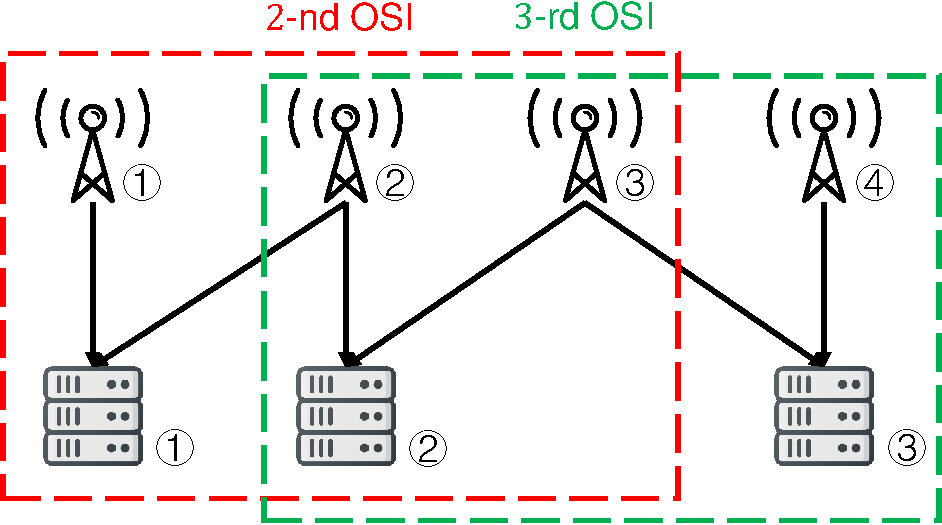
\includegraphics[width=1.0\textwidth]{chapter3/osi-example.pdf}
    \caption{An example of system model, where the edge servers $1,2,3$ are collocated with the APs $1,2,4$, respectively.}
    \label{fig:osi_example}
\end{figure*}

\begin{example}
    As illustrated in \figurename~\ref{fig:osi_example}, there are four APs and three edge servers collocated with the APs, in the edge computing system, where the solid directed lines show all the possible job dispatching paths for the APs.
    For the $2$-nd AP, its OSI includes the state information of the APs indexed with $1,3$ and the edge servers indexed with $1,2$.
    The state information of the $3$-rd edge server is out of its scope.
    
    Moreover, the OSI of the $3$-rd AP (namely, the $3$-rd OSI) includes the state information of the APs indexed with $2,4$ and the edge servers indexed with $2,3$.
    Note that the prediction of future state distribution is essential for solving the RHS of Equation (\ref{eqn:sp_0}).
    Without GSI, it is impossible to predict the future dispatching decisions of the $3$-rd AP from the perspective of the $2$-nd AP, since they observe different OSIs.
    It is thereby impossible for the $2$-nd AP to predict the future state distributions of the $2$-nd edge server, lack of the dispatching decisions of the $3$-rd AP.
    As a result, the evaluation of optimal value function of Equation (\ref{eqn:val_f}) is infeasible at both $2$-nd and $3$-rd APs, and the distributed policy optimization for them is a POMDP.
\end{example}

The general solution of POMDP is of huge complexity {as all the historical system states should be traced back in the current system state} \cite{IJCAI03-NairR,IJCAI99-BoutilierC}.
In this chapter, we shall propose a novel low-complexity solution framework based on an analytical approximation of the value function $V(\cdot)$ and alternative actions update, where distributed job dispatching via the Bellman's equations becomes feasible
(the minimization at the RHS of Equation (\ref{eqn:sp_0}) is solvable with the approximate value function)
even with OSI and local {\brlatency}.

%=================================================================================================%
%=================================================================================================%

\section{A Distributed Solution Framework with Partial Information}
\label{sec:chapter3-algorithm}
In this section, we shall propose a novel approximation framework, called {\Dalgname}, to decouple the centralized optimization on the RHS of the Bellman's equations in Equation (\ref{eqn:sp_0}) to each AP for arbitrary system state.
For the APs outside $\ccSet_{k}$, i.e., the conflict AP set of the $k$-th AP, the update of their dispatching actions will not affect the task computation originated from the $k$-th AP ($\forall k\in\apSet$).
Thus, the optimization of their dispatching actions can be decoupled.
However, for the APs within the same conflict AP set, the optimization of their dispatching actions is coupled.
Due to the unknown signaling latency, it is difficult for one AP (say the $k$-th AP) to predict the update of the dispatching actions at the other APs ($\forall k' \in\ccSet_{k}$).
Hence, cooperative optimization of dispatching actions for the APs within the same conflict AP set is difficult.

To this end, we introduce an \emph{alternative policy iteration algorithm}, to alternatively optimize the dispatching actions of one AP in a conflict AP set in each broadcast interval, while other APs maintain their dispatching actions in the previous broadcast interval.
Specifically, the proposed distributed algorithm consists of the following two steps:
\begin{enumerate}
    \item We first introduce a baseline policy, use its value function to approximate the value function of the optimal policy $\Policy^*$, and derive the analytical expression of the approximate value function for arbitrary GSI in Section \ref{subsec:chapter3-baseline}.
    \item With the approximate value function, in Section \ref{subsec:chapter3-ap_alg}, the AP set is partitioned into multiple independent subsets,
    %an alternative action update algorithm
    and only one out of these subsets is selected to update dispatching actions distributedly in each broadcast interval.
    Moreover, both analytical and semi-analytical performance bounds are derived in Section \ref{subsec:chapter3-analysis}.
\end{enumerate}
As a remark notice that solving the value function and then the RHS of the Bellman's equations are the two standard steps to solve an MDP problem with complete knowledge of the system state.
In our proposed solution framework, we extend this procedure to the POMDP problem in P1 by exploiting the structure of partially connected edge computing systems.
To the best knowledge of authors, a POMDP can hardly be solved via the Bellman's equations of full system state knowledge in the existing literature.

\subsection{Baseline Policy and Approximate Value Function}
\label{subsec:chapter3-baseline}
To alleviate the curse of dimensionality, we first use the baseline policy $\Baseline$ with fixed dispatching actions to approximate the value function at the RHS of the Bellman's equations in Equation (\ref{eqn:val_f}).
Specifically, the baseline policy we used is elaborated below.

\begin{definition}[Baseline Policy]
    In the baseline policy $\Baseline$, each AP fixes the target processing edge server for each job type as the previous broadcast interval. Specifically, at the $t$-th broadcast interval,
    \begin{align}
        \Baseline\Paren{\Stat(t),\Delay(t)} &\define \Brace{ 
            \Pi_{1}(\Stat_{1}(t),\mathcal{D}_{1}(t)),
            \dots,
            \Pi_{K}(\Stat_{K}(t),\mathcal{D}_{K}(t))
        },
    \end{align}
    where the baseline policy of the $k$-th AP $\Pi_k$ is given by 
    \begin{align}
        \Pi_{k}\Paren{\Stat_{k}(t),\mathcal{D}_{k}(t)}
        &= \Brace{
            {\omega}_{k,j}(t+1) \Big| \forall j\in\jSpace
        }, \forall k\in\apSet,
    \end{align}
    and $\omega_{k,j}(t+1) = \omega_{k,j}(t)$.
\end{definition}

Let $W_{\Baseline}(\cdot)$ be the value function of the baseline policy $\Baseline$, we shall approximate the value function of the optimal policy $V(\cdot)$ via $W_{\Baseline}$, i.e.,
\begin{align}
    V\Paren{\Stat(t+1)} &\approx W_{\Baseline}\Paren{\Stat(t+1)}
    \nonumber\\
    &= \sum_{m\in\esSet,j\in\jSpace}\Brace{
        \sum_{k\in\apSet} \tilde{W}^{\AP}_{k,m,j}(\Stat(t+1))
        +\tilde{W}^{\ES}_{m,j}(\Stat(t+1))
    },
    \label{eqn:baseline}
\end{align}
where $\tilde{W}^{\AP}_{k,m,j}(\Stat(t+1))$ denotes the cost raised by the type-$j$ jobs which are being transmitted from the $k$-th AP to the $m$-th edge server with baseline policy $\Baseline$ and system state $\Stat(t+1)$, and $\tilde{W}^{\ES}_{m,j}(\Stat(t+1))$ denotes the cost raised by the type-$j$ jobs on the $m$-th server.
Their definitions are given below.
\begin{align}
    \tilde{W}^{\AP}_{k,m,j} \Paren{\Stat(t+1)} &\define
        \sum_{i=0}^{\infty} \gamma^{i+1} \mathbb{E}^{\Baseline}\Bracket{
            \Inorm{\vec{R}^{(k)}_{m,j}(t+i+1)}
        },
    \\    
    \tilde{W}^{\ES}_{m,j} \Paren{\Stat(t+1)} &\define
        \sum_{i=0}^{\infty} \gamma^{i+1} \mathbb{E}^{\Baseline}\Bracket{
            Q_{m,j}(t+i+1) +
            \nonumber\\
            &~~~~~~~~~~~~~~~~~~~~\beta I[Q_{m,j}(t+i+1) = L_{max}]
        }.
\end{align}

Moreover, the analytical expressions of $\tilde{W}^{\AP}_{k,m,j}(\Stat(t+1))$ and $\tilde{W}^{\ES}_{m,j}(\Stat(t+1))$ are derived in the following lemmas, respectively.

\begin{lemma}[Analytical Expression of $\tilde{W}^{\AP}_{k,m,j}$]
    \label{lemma:w_ap}
    \begin{align}
        &\tilde{W}^{\AP}_{k,m,j}\Paren{\Stat(t+1)} =
        \bigg\|
            \vecG{\Theta}^{(k, \Baseline)}_{m,j}(t+1) \times
            \Bracket{
                \mat{I} - \gamma \Gamma^{(k)}_{m,j}
            }^{-1}
        \bigg\|,
        \label{w_ap}
    \end{align}
    where $\mat{I}$ is the identity matrix, and $\vecG{\Theta}^{(k, \Baseline)}_{m,j}(t)$ and $\Gamma^{(k)}_{m,j}$ are defined below.
    \begin{itemize}
        \item $\vecG{\Theta}^{(k,\Baseline)}_{m,j}(t) \define \Bracket{
            \theta^{(k,\Baseline)}_{m,j}(0,t),
            \theta^{(k,\Baseline)}_{m,j}(1,t),
            \dots,
            \theta^{(k,\Baseline)}_{m,j}(\Xi,t)
            }$,
        where 
        \begin{align*}
            \theta^{(k,\Baseline)}_{m,j}(\xi,t) \define 
            \begin{cases}
                \lambda_{k,j} I[\omega_{k,j}(t)=m], & \xi=0
                \\
                R^{(k)}_{m,j} = 1, & \text{otherwise}
            \end{cases}
        \end{align*}
        denotes the probability that there is one type-$j$ job have been delivered from $k$-th AP to $m$-th edge server for $\xi$ time slots at the very beginning of the $t$-th broadcast interval, when the baseline policy $\Baseline$ is adopted;
        \item $\Gamma^{(k)}_{m,j} \in \mathbb{R}^{(\Xi+1)\times(\Xi+1)}$ denotes the transition matrix of $\vecG{\Theta}^{(k,\Baseline)}_{m,j}(t)$ ($\forall t$) under baseline policy $\Baseline$ whose entries are provided in the following proof.
    \end{itemize}
\end{lemma}
\begin{proof}
    At the $n$-th time slot of the $t$-th broadcast interval, let $\hat{\vecG{\Theta}}^{(k,\Policy)}_{m,j}(t,n)$ denote the probability vector of job existence under dispatching policy $\Policy$, of which the explicit definition is given as follows.
    \begin{align}
        \hat{\vecG{\Theta}}^{(k,\Policy)}_{m,j}(t,n) \define \Bracket{
            \hat{\theta}^{(k,\Policy)}_{m,j}(0,t,n),
            \dots,
            \hat{\theta}^{(k,\Policy)}_{m,j}(\Xi,t,n)
        },
    \end{align}
    where
    \begin{align}
        \hat{\theta}^{(k,\Policy)}_{m,j}(\xi,t,n) \define
        \begin{cases}
            \lambda_{k,j} I[\omega_{k,j}(t)=m], &\xi=0, n < \mathcal{D}_{k}(t)
            \\
            \lambda_{k,j} I[\omega_{k,j}(t+1)=m], &\xi=0, n \geq \mathcal{D}_{k}(t) 
            \\
            \Pr\{R^{(k)}_{m,j}(\xi,t,n)=1\}, & \text{otherwise}
        \end{cases}
    \end{align}
    denotes the probability that $\xi$ jobs are in uploading from the $k$-th AP to the $m$-th edge server under dispatching policy $\Policy$, at the $n$-th time slot of the $t$-th broadcast interval.
    The dispatching policy $\Policy$ only affects the first entry of the probability vector, i.e., the arrival probability of one job in the time slot.
    Hence, we denote the time-invariant and policy-independent transition matrix $\hat{\Gamma}^{(k)}_{m,j}$ for the state transition on AP between adjacent time slots, which is defined as follows.
    \begin{align}
        \hat{\Gamma}^{(k)}_{m,j} &\define
        \begin{bmatrix}
            1 & \bar{p}^{(k)}_{m,j,0} &                       &        &                           \\
            & 0                     & \bar{p}^{(k)}_{m,j,1} &        & \text{\huge0}             \\
            &                       & \ddots                & \ddots &                           \\
            & \text{\huge0}         &                       & \ddots & \bar{p}^{(k)}_{m,j,\Xi-1} \\
            &                       &                       &        & 0                         \\
        \end{bmatrix},
    \end{align}
    where $\bar{p}^{(k)}_{m,j,\xi}$ denotes the probability of job still staying at the $k$-th AP in the next time slot as $\bar{p}^{(k)}_{m,j,\xi} = 1 - p^{(k)}_{m,j,\xi}$, and
    \begin{align}
        p^{(k)}_{m,j,\xi} &\define \Pr\{U^{(k)}_{m,j} < (\xi+1) | U^{(k)}_{m,j}>\xi\}
    \end{align}
    denotes the probability of job offloading to the $m$-th edge server.

    Hence, let ${\vecG{\Theta}}^{(k, \Policy)}_{m,j}(t)$ and ${\Gamma}^{(k)}_{m,j}$ denotes the probability vector and transition matrix for the adjacent broadcast intervals, respectively.
    Based on the previous definitions at the scale of time slot, the expressions of $\vecG{\Theta}^{(\Policy, k)}_{m,j}(t)$ and the transition process between adjacent broadcast intervals under policy $\Policy$ are given as follows.
    \begin{align}
        \vecG{\Theta}^{(k, \Policy)}_{m,j}(t) &\define \hat{\vecG{\Theta}}^{(k, \Policy)}_{m,j}(t,0),
        \\
        \vecG{\Theta}^{(k, \Policy)}_{m,j}(t+1) &= \hat{\vecG{\Theta}}^{(k, \Policy)}_{m,j}(t, \mathcal{D}_{k}(t)) \times (\hat{\Gamma}^{(k)}_{m,j})^{t_B-\mathcal{D}_{k}(t)},
        \nonumber\\
        \hat{\vecG{\Theta}}^{(k, \Policy)}_{m,j}(t, \mathcal{D}_{k}(t)) &= \vecG{\Theta}_{m,j}(t) \times (\hat{\Gamma}^{(k, \Policy)}_{m,j})^{\mathcal{D}_{k}(t)}.
    \end{align}
    Given that the cost raised on APs are approximated via baseline policy $\Baseline$, the AP (saying the $k$-th AP) would adopt the same dispatching actions as $\Pi_{k}(\Stat_{k}(t), \mathcal{D}_{k}(t))$ before and after $\mathcal{D}_{k}(t)$ time slots at the $t$-th broadcast interval.
    Hence, we have
    \begin{align}
        \vecG{\Theta}^{(k,\Baseline)}_{m,j}(t+1) = \vecG{\Theta}^{(k,\Baseline)}_{m,j}(t) \times (\hat{\Gamma}^{(k)}_{m,j})^{t_B}.
    \end{align}
    and the definition of transition matrix $\Gamma^{(k)}_{m,j}$ with baseline policy $\Baseline$ as
    \begin{align}
        \Gamma^{(k)}_{m,j} &\define \big( \hat{\Gamma}^{(k)}_{m,j} \big)^{t_B}.
    \end{align}
    Hence, the expression of the cost raised on the AP (say the $k$-th AP) under baseline policy $\Baseline$ is given as follows.
    \begin{align}
        &\tilde{W}^{\AP}_{k,m,j}\Paren{\Stat(t+1)} =
        \Inorm{
            \vecG{\Theta}^{(k, \Baseline)}_{m,j}(t+1) \times
            \Bracket{
                \mat{I} - \gamma \Gamma^{(k)}_{m,j}
            }^{-1}
        }.
    \end{align}
\end{proof}

\begin{lemma}[Analytical Expression of $\tilde{W}^{\ES}_{m,j}$]
    \label{lemma:w_es}
    \begin{align}
    \tilde{W}^{\ES}_{m,j}\Paren{\Stat(t+1)}
    = &\sum_{i=0,\dots,\frac{\Xi}{T}} \gamma^{i} \mathbb{E}^{\Baseline}[ Q_{m,j}({t+i+1}) | \Stat(t+1)]
    \nonumber\\
    &+ \gamma^{\frac{\Xi}{T}} 
    \vecG{\nu}_{m,j}({t+\frac{\Xi}{T}+1})
    \Paren{
        \mat{I} - \gamma \mat{P}^{\Baseline}_{m,j}(t+\frac{\Xi}{T}+1)
    }^{-1} \vec{g}',
        \label{w_es}
    \end{align}   
    where $\vecG{\nu}_{m,j}(t)$, $\mat{P}_{m,j}(\beta_{m,j}(t))$, $\beta_{m,j}(t)$ and $\vec{g}$ are defined below.
    \begin{itemize}
        \item
        $\vecG{\nu}_{m,j}(t) \define [\Pr\{Q_{m,j}(t)=0\}, \dots, \Pr\{Q_{m,j}(t)=L_{max}\}]$
        denotes the PMF (probability mass function) vector of $Q_{m,j}(t)$.
        \item $\vec{g} \in \mathbb{R}^{(L_{max}+1) \times 1}$ denotes the cost vector of edge server, and its $i$-th entry is
        \begin{align}
            [\vec{g}]_{i} \define 
            \begin{cases}
                i, & i=0,1,\dots,L_{max}-1
                \\
                L_{max}+\beta, & \text{otherwise}
            \end{cases}.
            \label{eqn:g_vec}
        \end{align}
        \item The expression of $\mathbb{E}^{\Baseline}[ Q_{m,j}({t+i+1}) | \Stat(t+i)]$ is elaborated in the following proof.
        \item $\mat{P}^{\Baseline}_{m,j}(t) \in \mathbb{R}^{(L_{max}+1) \times (L_{max}+1)}$ denotes the transition matrix of $\vecG{\nu}_{m,j}(t)$ under baseline policy $\Baseline$ whose entries are described in the following proof.
    \end{itemize}
\end{lemma}
\begin{proof}
    The state transition on edge server is composed of both arrival processes of all the APs in the corresponding \emph{potential AP set}, and the departure processes of jobs computation.
    We first denote the offloading matrix $\bar{\Gamma}^{(k)}_{m,j}$ for the type-$j$ job offloaded from the $k$-th AP to the $m$-th edge server and the offloading probability vector $\vecG{\rho}^{(k)}_{m,j}({t,n})$ as follows, respectively ($\forall k\in\apSet, m\in\esSet_{k}, j\in\jSpace$).
    \begin{align}
        \bar{\Gamma}^{(k)}_{m,j}(t,n) &\define
        \begin{bmatrix}
            0 & p^{(k)}_{m,j,0} &                 &        &                     \\
            & 0                 & p^{(k)}_{m,j,1} &        & \text{\huge0}       \\
            &                   & \ddots          & \ddots &                     \\
            & \text{\huge0}     &                 & \ddots & p^{(k)}_{m,j,\Xi-1} \\
            &                   &                 &        & 1                   \\
        \end{bmatrix},
        \\
        \vecG{\rho}^{(k, \Policy)}_{m,j}({t,n}) &\define \hat{\vecG{\Theta}}^{(k, \Policy)}_{m,j}({t,n}) \times \bar{\Gamma}^{(k)}_{m,j}.
    \end{align}

    However, the computational complexity of combinations of all the offloading probability vectors for the $m$-th edge server from its \emph{potential AP set} is unacceptable.
    To alleviate the complexity, we rewrite the combinatorial arrival process on edge server as an equivalent Bernoulli process with \emph{small probability approximation}, i.e., there would be at most one job arriving in one time slot with the probability as the expected arrival rate of the original combinatorial distribution.
    Specifically, the probability distribution of $\sum_{k\in\apSet_{m}} \vecG{\rho}^{(k, \Policy)}_{m,j}({t,n})$ is approximated as a Bernoulli distribution with the expected arrival rate denoted as $\hat{\beta}^{\Policy}_{m,j}({t,n})$ whose definition is given as
    \begin{align}
        \hat{\beta}^{\Policy}_{m,j}({t,n}) &\define \sum_{k\in\apSet_{m}} \sum_{\xi=0,\dots,\Xi-1} \mathbb{E}[\vecG{\rho}^{(k, \Policy)}_{m,j,\xi}({t,n})].
    \end{align}

    %NOTE: transition matrix and vector for Edge Server
    Let $\hat{\vecG{\nu}}_{m,j}(t,n)$ denote the probability vector of $Q_{m,j}(t,n)$ at the $n$-th time slot of the $t$-th broadcast interval ($\forall m\in\esSet, j\in\jSpace$)
    \begin{align}
        \vecG{\nu}_{m,j}(t,n) \define \Bracket{
            \Pr\{Q_{m,j}(t,n)=0\}, \dots, \Pr\{Q_{m,j}(t,n)=L_{max}\}
        }.
    \end{align}
    The transition matrix $\hat{\mat{P}}_{m,j}(\hat{\beta}^{\Policy}_{m,j}(t,n))$ for adjacent time slots is determined by $\hat{\beta}^{\Policy}_{m,j}(t,n)$ under policy $\Policy$, whose entries are elaborated as follows.
    \begin{align}
        &\Bracket{ \hat{\mat{P}}_{m,j}(\hat{\beta}^{\Policy}_{m,j}(t,n)) }_{a,b} =
        \nonumber\\
        &~~~~~~\begin{cases}
            (1/c_{m,j})(1-\hat{\beta}^{\Policy}_{m,j}(t,n)), & b=a-1 \\
            (1-1/c_{m,j})\hat{\beta}^{\Policy}_{m,j}(t,n), & b=a+1 \\
            (1/c_{m,j})\hat{\beta}^{\Policy}_{m,j}(t,n) + (1-1/c_{m,j})(1-\hat{\beta}^{\Policy}_{m,j}(t,n)), & a=b \\
            0, &\text{otherwise}
        \end{cases}.
    \end{align}

    Hence, let $\vecG{\nu}_{m,j}(t)$ and $\mat{P}^{\Policy}_{m,j}(t)$ denote the probability vector and transition matrix for adjacent broadcast intervals, respectively.
    Based on the previous definitions in the time slot, the explicit definition is given as
    \begin{align}
        \vecG{\nu}_{m,j}(t) &\define \hat{\vecG{\nu}}_{m,j}(t,0)
        \\
        \mat{P}^{\Policy}_{m,j}(t) &\define \prod_{n=0,\dots,t_B-1} \hat{\mat{P}}_{m,j}(\hat{\beta}^{\Policy}_{m,j}(t,n)),
        \\
        \vecG{\nu}_{m,j}(t+1) &= \vecG{\nu}_{m,j}(t) \times \mat{P}^{\Policy}_{m,j}(t)
    \end{align}

    Given that the cost raised on edge servers is approximated with baseline policy $\Baseline$, the transition matrix for state transition is affected by the baseline policy and the system states of APs which could not be decoupled.
    \begin{align}
        \mathbb{E}^{\Baseline}[ Q_{m,j}({t+i+1}) | \Stat(t+i)] &\define
            \vecG{\nu}_{m,j}(t) \mat{P}^{\Baseline}_{m,j}(t+i) \vec{h}',
    \end{align}
    where $\vecG{h} \define [0,1,\dots,L_{max}]$.

    Moreover, we notice that under the fixed baseline policy, the arrival process on edge servers would be stationary after the maximum uploading latency from the initial interval and thus the transition matrix is invariant of system states of APs.
    Let $\hat{\mat{P}}_{m,j}(\hat{\beta}^{\Baseline}_{m,j}(t,n))$ be the transition matrix for the stationary arrival process under baseline policy $\Baseline$ and
    \begin{align}
        \beta_{m,j}(t,n) &\define \sum_{k\in\apSet} \lambda_{k,j}I[\omega_{k,j}(t)=m] \times \Pr\{ \xi<U_{k,m,j}\le\xi+1 \}
        \nonumber\\
        &= \sum_{k\in\apSet} \lambda_{k,j}I[\omega_{k,j}(t)=m]\ (\forall n),
    \end{align}
    where $U_{k,m,j}$ denotes the random variable of job uploading latency (with the unit of time slot).

    Let
    $\mat{P}^{\Baseline}_{m,j}(t) \define \big( \hat{\mat{P}}_{m,j}(\hat{\beta}^{\Baseline}_{m,j}(t,n)) \big)^{t_B}$
    denote the transition matrix under baseline policy $\Baseline$ between adjacent broadcast intervals, we could express the cost raised on edge server under baseline policy $\Baseline$ as follows.
    \begin{align}
        &\tilde{W}^{\ES}_{m,j}\Paren{\Stat(t+1)}
        = \sum_{i=0,\dots,\frac{\Xi}{T}} \gamma^{i} \mathbb{E}^{\Baseline}[ Q_{m,j}({t+i+1}) ]
        \nonumber\\
        &~~~~~~~~~~~~+ \gamma^{\frac{\Xi}{T}} 
        \vecG{\nu}({t+\frac{\Xi}{T}+1})
        \Paren{
            \mat{I} - \gamma \mat{P}^{\Baseline}_{m,j}(t)
        }^{-1} \vec{g}',
    \end{align} 
    where $\vec{g}$ is the cost vector whose definition is given in Equation (\ref{eqn:g_vec}).
\end{proof}

\subsection{Distributed Action Update}
\label{subsec:chapter3-ap_alg}
Although the optimal value function has been approximated via the baseline policy in the previous part, it is still infeasible for all the APs to solve the RHS of the Bellman's equations in a distributed manner with OSI and local {\brlatency} only.
This is because the evaluation of Equations (\ref{w_ap}) and (\ref{w_es}) requires the knowledge of GSI and {\brlatency} at all APs.
Instead, it is feasible for part of APs to update their dispatching actions distributedly in each broadcast interval and achieve a better performance compared with baseline policy.
Hence, we first define the following collection of AP subsets, namely \emph{AP partition}, where one subset is selected to update dispatching actions in one broadcast interval, and all the subsets are selected alternatively for different broadcast {intervals}.
\begin{definition}[AP Partition]
    A collection of AP subsets $(Y_1, \dots, Y_N)$ is named as AP partition, if $\mathcal{Y}_{1}, \dots, \mathcal{Y}_{N} \subseteq \apSet$ and
    \begin{align}
        &\bigcup_{n=0,\dots,N-1} \mathcal{Y}_{n} = \apSet
        \label{eqn:subset_cup}
        \\
        \esSet_{y} \cap \esSet_{y'} &=\emptyset, y' \neq y~(\forall y',y \in \mathcal{Y}_{n}).
        \label{eqn:subset_disjoint}
    \end{align}
\end{definition}

The condition in Equation (\ref{eqn:subset_cup}) is to ensure all the APs can update their dispatching actions periodically; whereas the condition in Equation (\ref{eqn:subset_disjoint}) is to ensure APs in the conflict AP sets of each other will not update their dispatching actions in the same broadcast interval.
For example, as illustrated in \figurename~\ref{fig:system}, the AP set $\apSet$ could be decomposed of three subsets as $\set{1,3,4}$, $\set{2}$ and $\set{5}$.
The subset partition is not trivial and a partition minimizing the update period $N$ is preferred.
A heuristic greedy algorithm is given in Algorithm \ref{alg_0}.
\begin{algorithm}[ht]
    \caption{Greedy Subset Partition Algorithm}\label{alg_0}
    \DontPrintSemicolon
    \KwIn{$\apSet, \set{\esSet_{k}, \forall k\in\apSet}$ }
    \KwOut{a subset partition $\set{ \mathcal{Y}_{n} }$}
    Initialize the subset partition as $\mathcal{Y}_{n} = \set{n}$ ($\forall n\in\apSet$).\;
    \While{ $\exists \mathcal{Y}_a$ and $\mathcal{Y}_b$ ($a \neq b$), $\bigcup_{y\in\mathcal{Y}_a}\esSet_{y} \cap \bigcup_{y\in\mathcal{Y}_{b}} \esSet_{y} = \emptyset$ }
    {
        Count number of subsets in the current subset partition which have disjoint candidate set with $\mathcal{Y}_n$ ($\forall n$), denoted the number as $I_{n}$.\;
        $\tilde{n} \gets \arg\min_{n} I_{n}$\;
        Merge the subset $Y_{\tilde{n}}$ with one of its disjoint subsets.\;
    }
\end{algorithm}

At the $t$-th broadcast interval, the APs in the subset indexed with $n \define t \mod{N}$ update their dispatching actions, while the other APs keep the same dispatching actions as the previous broadcast interval.
Hence, let
\begin{align}
    \tilde{\mathcal{A}}(t) \define \Brace{ {\omega}_{y,j}(t+1) \Big| \forall y\in\mathcal{Y}_{n},j\in\jSpace }
\end{align}
be the aggregation of dispatching actions of the APs in the subset $\mathcal{Y}_{n}$, and
\begin{align}
    \hat{\mathcal{A}}(t) \define \Brace{ {\omega}_{y,j}(t+1) \Big| \forall y\notin\mathcal{Y}_{n}, j\in\jSpace}
\end{align}
be the aggregation of dispatching actions of the rest APs, which are the same as the previous broadcast interval.
At the $t$-th broadcast interval, the optimization of $\tilde{\mathcal{A}}(t)$ at the RHS of the Bellman's equations can be rewritten as the following problem.
\begin{align}
    \textbf{P2:}~
    \min_{ \tilde{\mathcal{A}}(t) }
    &\sum_{\Stat(t+1)} \Pr\Brace{
        \Stat(t+1) \Big| \Stat(t), \hat{\mathcal{A}}(t), \tilde{\mathcal{A}}(t)
    } \cdot W_{\Baseline}\Paren{\Stat(t+1)}.
\end{align}

Moreover, we have the following conclusion on the decomposition of P2.
\begin{lemma}[]
    The optimization problem in P2 can be equivalently decoupled into local optimization problems at APs in $\mathcal{Y}_n$.
    Specifically, {the local optimization for each AP (say the $y$-th AP) in $\mathcal{Y}_n$ can be written as}
    \begin{align}
        \textbf{P3:}~
        \min_{ \tilde{\mathcal{A}}(t+1) }
        &\mathbb{E}_{\set{ \Stat_{y}(t+1)|\Stat_{y}(t), \tilde{\mathcal{A}}(t+1),\hat{\mathcal{A}}(t+1) }}
        \nonumber\\
        &\sum_{j\in\jSpace}
        \Brace{
            \tilde{W}^{\AP}_{y,m,j}\Paren{\Stat_{y}(t+1)}
            + \sum_{m\in\tilde{\esSet}_{y}} \tilde{W}^{\ES}_{m,j}\Paren{\Stat_{y}(t+1)}
        },
        \label{eqn:partial}
    \end{align}
    where \footnote{In Equation (\ref{eqn:baseline}), the costs $W^{\AP}_{y,m,j}(\Stat(t+1))$ and $W^{\ES}_{m,j}(\Stat(t+1))$ are expressed as a function of global system state $\Stat(t+1)$. In fact, these two costs can be completely determined by the OSI of the $y$-th AP as in Equation (\ref{eqn:partial}). Hence, we use the notations $W^{\AP}_{y,m,j}(\Stat_y(t+1))$ and $W^{\ES}_{m,j}(\Stat_y(t+1))$ instead.}
    \begin{align*}
       \tilde{\esSet}_{y} &= \set{\omega_{y,j}(t), \omega_{y,j}(t+1) | \forall j\in\jSpace}.
    \end{align*}
    \label{lemma:w_partial}
\end{lemma}
\begin{proof}
    At the $t$-th broadcast interval, the $y$-th AP in the subset $\mathcal{Y}_{n}$ updates its dispatching actions, which could only affect the future cost raised on itself and its corresponding \emph{candidate server set}, i.e., the part of its OSI.
    Hence, it's obvious that the expression of Equation (\ref{w_ap}) and Equation (\ref{w_es}) on the RHS of the Bellman's equations could be reduced into the form based only on the OSI of the $y$-th AP ($\forall y\in\mathcal{Y}_{n}$).
\end{proof}

The optimization of dispatching actions $\tilde{\Policy}_{y}(\Stat(t),\Delay(t))$ for the $y$-th AP ($\forall y\in\mathcal{Y}_{n}$) in P3 could be achieved via searching all the edge servers in candidate edge server set $\esSet_{y}$, whose computational complexity is $O(J|\mathcal{M}_{y}|)$.
As a result, the overall algorithm of job dispatching, is elaborated in Algorithm \ref{alg_1}.
\begin{algorithm}[ht]
    \caption{{\Dalgname}: Online Alternative Actions Update Algorithm}\label{alg_1}
    \DontPrintSemicolon
    Initialize all the APs with heuristic dispatching actions $\set{{\omega}_{k,j}(0)|\forall k\in\apSet,j\in\jSpace}$.\;
    \For{$t=0,1,2,\dots$}{
        \tcc{Get the index of the subset to update at $t$.}
        $n \gets t \mod{N}$\;
        \tcc{Parallel update the actions of APs in the subset $\mathcal{Y}_{n}$.}
        \ForPar{$y \in \mathcal{Y}_{n}$}{
            \tcc{Each AP observes its LSI asynchronously.}
            The $y$-th AP observes $\Stat_{y}(t)$ after $\mathcal{D}_{y}(t)$.\;
            \tcc{Then update actions by solving P3.}
            Solve P3 with $\Stat_{y}(t), \mathcal{D}_{y}(t)$ and obtain optimized actions $\set{\tilde{\omega}_{y,j}(t+1)|\forall j\in\jSpace}$\;
        }
        $\tilde{\mathcal{A}}(t+1) \gets \set{\tilde{\omega}_{y,j}(t+1)|\forall y\in\mathcal{Y}_{n},j\in\jSpace}.$\;
        \tcc{The other APs fix the actions as the previous interval.}
        $\hat{\mathcal{A}}(t+1) \gets \hphantom{~~} \set{ {\omega}_{y,j}(t) | \forall y\in\mathcal{Y}_{n-1},j\in\jSpace }$\;
        $\hphantom{~~~~~~~~~~~~~~~~~} \cup \set{ {\omega}_{y,j}(t) | \forall y\notin\mathcal{Y}_{n-1},j\in\jSpace }$\;
    }
\end{algorithm}

Moreover, we use the following example to illustrate the procedure of Algorithm \ref{alg_1}.
\begin{example}
    \label{exp:update}
    Consider an edge computing system as \figurename~\ref{fig:system}, where the AP set $\apSet$ could be partitioned into three subsets which are denoted as $\mathcal{Y}_{0} = \set{1,3,4}$, $\mathcal{Y}_{1} = \set{2}$, and $\mathcal{Y}_{2} = \set{5}$, respectively.
    As illustrated in \figurename~\ref{fig:update_timeline}, in the $1$-st interval the APs in subset $\mathcal{Y}_{0}$ would update their dispatching actions by solving P3, respectively, while the APs in subset $\mathcal{Y}_{1}$ and $\mathcal{Y}_{2}$ fix their actions.
    Denote the aggregation of their dispatching actions as $\tilde{\mathcal{A}}(1)$ and $\hat{\mathcal{A}}(1)$, respectively.
    In the $2$-nd interval, the APs in subset $\mathcal{Y}_{0}$ and $\mathcal{Y}_{2}$ fix their actions which is denoted via $\hat{\mathcal{A}}(2)$, while 
    the AP in subset $\mathcal{Y}_{1}$ updates the dispatching action. %to $\tilde{\mathcal{A}}(2)$.
    In the $3$-rd interval, the APs in subset $\mathcal{Y}_{0}$ and $\mathcal{Y}_{1}$ fix their actions and the AP in subset $\mathcal{Y}_{2}$ updates the dispatching action.
    Hence, every AP {updates} its dispatching actions with period $N=3$.
    \begin{figure*}[htp!]
        \centering
        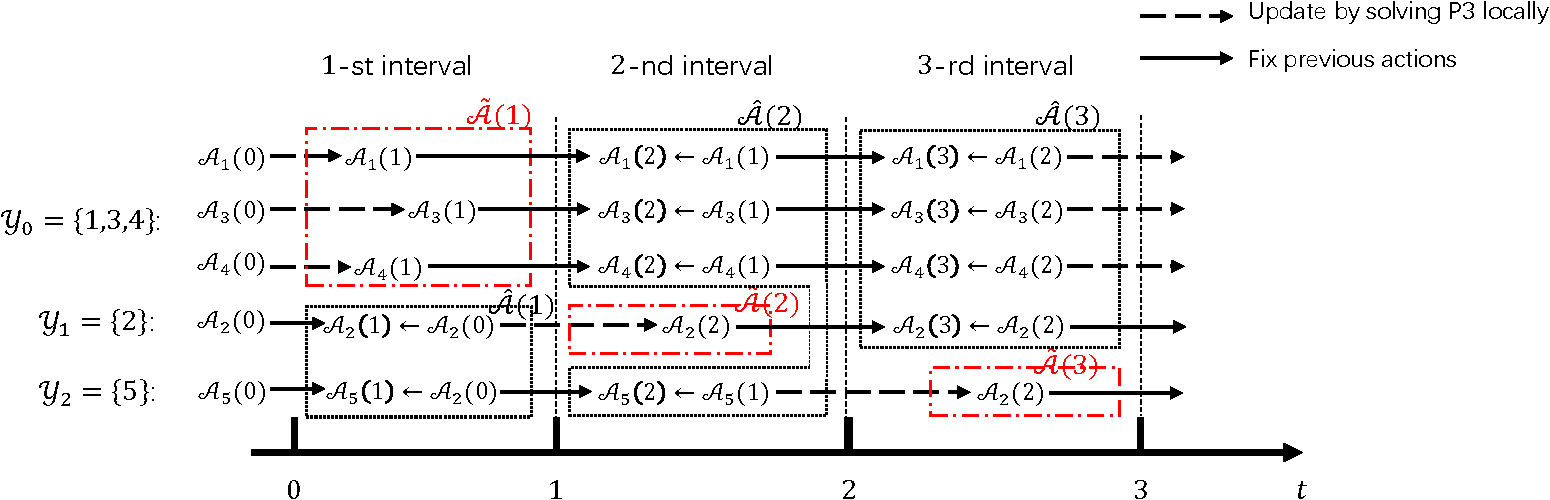
\includegraphics[width=1.0\textwidth]{chapter3/update-timeline.pdf}
        \caption{The Illustration of Example \ref{exp:update}.}
        \label{fig:update_timeline}
    \end{figure*}
\end{example}

As a remark notice that since in Algorithm \ref{alg_1}, the computation complexity at each AP scales linearly with respect to {the size of candidate edge server set}, it can be deployed in a scenario with massive APs and edge servers, as long as the {the number of candidate edge servers for each AP} is limited.

\subsection{Analytical and Semi-Analytical Performance Bounds}
\label{subsec:chapter3-analysis}
In most of the existing approximate MDP solutions \cite{mdp-bound1,mdp-bound2,mdp-bound3}, the performance is difficult to bound analytically as the approximate value function has no accurate meaning on the system cost or utility.
In the proposed algorithm, however, we derive the analytical expression for the baseline policy as the approximate value function.
The following lemma shows this analytical expression is a performance lower bound (cost upper bound) of our proposed policy (Algorithm \ref{alg_1}), {denoted as $\tilde{\Policy}(\Stat(t), \Delay(t))$}.
\begin{lemma}[Analytical Cost Upper Bound]
    \label{lemma:bound}
    Let $W_{\tilde{\Policy}}(\cdot)$ be the value function of the proposed policy $\tilde{\Omega}$, i.e.,
    \begin{align}
        W_{\tilde{\Policy}}(\Stat) \define
        \sum_{t=1}^{\infty} \gamma^{t-1} \mathbb{E}^{\tilde{\Policy}}_{\Delay} \Bracket{
            g\Paren{\Stat(t)} \Big| \Stat(1)=\Stat
        },
        \label{eqn:bound}
    \end{align}
    we have
    \begin{align}
        V(\Stat)
        \leq W_{\tilde{\Policy}}(\Stat)
        \leq W_{\Baseline}(\Stat),
        \forall \Stat.
    \end{align}
    We denote the \emph{$1$-step improved policy} as $\hat{\Baseline}$, which is an intermediate between the baseline policy and the proposed policy. Specifically, $\hat{\Baseline}$ would update the dispatching actions following the Algorithm \ref{alg_1} in the first interval (saying the $t$-th interval) (i.e., at the same time slot with same subset of APs), and then fixes the actions in the following intervals. The explicit definitions are given as follows.
    \begin{align}
        \hat{\Baseline}\Paren{\Stat(t), \Delay(t)} \define 
        \begin{cases}
            \tilde{\Policy}({\Stat(0), \Delay(0)}), &t=1
            \\
            \tilde{\Policy}({\Stat(1), \Delay(1)}), &\text{otherwise}
        \end{cases}.
    \end{align}
    Let $V_{\hat{\Baseline}}(\cdot)$ be the value function of the \emph{$1$-step improved policy} $\hat{\Baseline}$, i.e.,
    \begin{align}
        V_{\hat{\Baseline}}(\Stat) = \mathbb{E}_{\Delay}\Bracket{ g\Paren{\Stat(1)} + \gamma W_{\hat{\Baseline}}\Paren{\Stat(2)} | \Stat(1)=\Stat }.
    \end{align}
    Moreover, as the broadcast interval is random, it is hard to obtain closed-form analytical expression for the tight performance bound $V_{\hat{\Baseline}}(\Stat)$ and a semi-analytical method is proposed.
\end{lemma}
\begin{proof}
    Since the proposed policy $\tilde{\Policy}$ is not optimal policy and $W_{\tilde{\Policy}}(\Stat)$ represents the average system cost with the proposed policy $\tilde{\Policy}$, $V(\Stat) \leq W_{\tilde{\Policy}}(\Stat)$ is straightforward.
    Let 
    \begin{align*}
        \Delta(t) \triangleq &
        \sum_{t'=1}^{\infty} \gamma^{t'-1}
        \mathbb{E}^{ \tilde{\Policy} } \Bracket{
            g\Paren{\Stat(t'), \tilde{\Policy}(\Stat(t'),t-1)}
            -  g\Paren{\Stat(t'), \tilde{\Policy}(\Stat(t'),t)}
        }
    \end{align*}
    denote the improvement of the $t$-th policy update.
    According to Proposition 2.3.3 (a) in \cite{dp-control}, we have $\Delta(t)\geq 0$, $\forall t$.

    Hence, we have
    \begin{align*}
    W_{\Baseline}(\Stat)- W_{\tilde{\Policy}}(\Stat)
    &= 
    \underbrace{\sum_{t'=1}^{N} \gamma^{t'-1} \mathbb{E}^{ \tilde{\Policy} } \Bracket{
        g\Paren{\Stat(t'), \tilde{\Policy}(\Stat(t'),0)}
        - 	g\Paren{\Stat(t'), \tilde{\Policy}(\Stat(t'),t')}
    }}_{\mathfrak{F}(N)}\\
    &+\sum_{t'=N+1}^{+\infty} \gamma^{t'-1} \mathbb{E}^{ \tilde{\Policy} } \Bracket{
        g\Paren{\Stat(t'), \tilde{\Policy}(\Stat(t'),0)}
        - 	g\Paren{\Stat(t'), \tilde{\Policy}(\Stat(t'),t')}
    }\\
    &\geq \mathfrak{F}(N) + \underbrace{\sum_{t'=N+1}^{+\infty} \gamma^{t'-1} \mathbb{E}^{ \tilde{\Policy} } \Bracket{
        g\Paren{\Stat(t'), \tilde{\Policy}(\Stat(t'),0)}
        - 	g_{\max}
    }}_{\mathfrak{G}(N)},
    \end{align*}
    where $g_{\max}$ denotes the upper-bound of the per-stage cost $g(\cdot)$.
    Because  $\mathfrak{F}(N)=\sum_{t=1}^{N}\gamma^{t-1}\Delta(t)\geq 0$, $\mathfrak{F}(N)$ increases as $N$ increases.
    It is obvious that $\mathfrak{G}(N)$ increases as $N$ increases, and 
    \begin{align*}
    \lim\limits_{N\to+\infty}\mathfrak{G}(N)=0
    \end{align*}
    Hence, 
    \begin{align*}
    \exists N,\ \mbox{s.t. }\ W_{\Baseline}(\Stat)- W_{\tilde{\Policy}}(\Stat)\geq \mathfrak{F}(N)-\mathfrak{G}(N) \geq 0.
    \end{align*}
\end{proof}

The above cost upper bound $W_{\Baseline}(\Stat)$ is obtained by assuming all the APs fix the target edge servers for task computation.
Its gap to the performance of the proposed policy, denoted as $W_{\Baseline}(\Stat) - W_{\tilde{\Policy}}(\Stat)$, is mainly due to the adaptive job dispatching of the proposed policy.
Therefore, a tighter semi-analytical cost upper bound is provided below which could be used for quick performance evaluation.
\begin{lemma}[Semi-Analytical Cost Upper Bound]
    Let $\hat{\Baseline}^{(T)}$ denote an intermediate policy, which follows $\tilde{\Policy}$ in the first $T$ intervals and then fixes the policy at the $T$-th interval in the following intervals ($T$ is an arbitrary positive integer), then
    \begin{align}
        W_{\tilde{\Policy}}(\Stat) \leq W_{\hat{\Baseline}}^{(T)}(\Stat)
        \define &\sum_{t=1}^{T} \gamma^{t-1} \mathbb{E}^{\tilde{\Policy}}_{\Delay}\Bracket{g\Paren{\Stat(t)} | \Stat(1)=\Stat}
        \nonumber\\
        &+\gamma^{T} \mathbb{E}^{\Baseline}_{\Stat(T+1)}\Bracket{W_{\Baseline}\Paren{\Stat(T+1)}}.
        \label{eqn:semi-bound}
    \end{align}
    Moreover, the gap $e(T) = W^{(T)}_{\hat{\Baseline}}(\Stat) - W_{\tilde{\Policy}}(\Stat)$ is monotonically decreasing with respect to $T$.
\end{lemma}
\begin{proof}
    Firstly, it is obvious that $W^{(T)}_{\hat{\Baseline}}(\Stat)$ is the cost upper bound for the proposed policy $\tilde{\Policy}$.
    As the Equation (\ref{eqn:bound}) could be split into two parts as shown below,
    \begin{align*}
        W_{\tilde{\Policy}}(\Stat) =
        \sum_{t=1}^{T} &\gamma^{t-1} \mathbb{E}^{\tilde{\Policy}}_{\Delay} \Bracket{ g\Paren{\Stat(t)} | \Stat(1)=\Stat }
        +
        \nonumber\\
        &\gamma^{T} \sum_{t=1}^{\infty} \gamma^{t-1} \mathbb{E}^{\tilde{\Policy}}_{\Delay,\Stat(T+1)} \Bracket{ g\Paren{\Stat(t+T)} },
    \end{align*}
    where the first part is exactly same as the first part in Equation \eqref{eqn:semi-bound} of $W^{(T)}_{\hat{\Baseline}}(\Stat)$, and the second part $\sum_{t=1}^{\infty}\gamma^{t-1}\mathbb{E}^{\tilde{\Policy}}_{\Delay}[g(\Stat(t+T))]$ is upper bounded by $W_{\Baseline}(\Stat(T+1))$ as illustrated in the proof given in lemma \ref{lemma:bound}.

    Then, we show that the performance gap $e(T)$ monotonically decreases with respect to $T$.
    For any positive integer $T$, let
    \begin{align*}
        \Delta{W}(T) \define W^{(T+1)}_{\hat{\Baseline}}(\Stat) - W^{(T)}_{\hat{\Baseline}}(\Stat)
    \end{align*}
    denotes the performance gap due to one-step policy improvement described in Equation (\ref{eqn:partial}).
    According to the \emph{Proposition 2.3.4 (Cost Improvement by Rollout)} in \cite{dp-control}, we have $W^{(T+1)}_{\hat{\Baseline}}(\Stat) \leq W^{(T)}_{\hat{\Baseline}}(\Stat)$ for all $\Stat$.
    Hence, we have $\Delta{W}(T) \geq 0$ for all $T$ and the performance gap $e(T)$ decreases monotonically with respect to $T$.
\end{proof}
In the above cost upper bound, the first item $\sum_{t=1}^{T} \gamma^{t-1} \mathbb{E}^{\tilde{\Policy}}_{\Delay}[g(\Stat(t))]$ has to be evaluated numerically, but the second item $\mathbb{E}^{\Baseline}_{\Stat(T+1)}[{W_{\Baseline}(\Stat(T+1))}]$ can be calculated analytically according to Lemma \ref{lemma:bound}.
The performance of both cost upper bounds will be illustrated in the following simulation section.

%=================================================================================================%
%=================================================================================================%

\section{Reinforcement Learning Algorithm}
\label{sec:chapter3-rl-alg}
Although the approximate value function $W_{\Baseline}(\Stat)$ is derived analytically in the previous section, the calculation of $ W_{\Baseline}(\Stat)$ requires the priori knowledge on the distributions in this system, i.e., the distributions of job arrival, uploading latency and computation time, are usually unknown in advance.
Therefore, we extend the {\Dalgname} with an efficient reinforcement learning approach.
Specifically, with the explicit analytical expressions of $\tilde{W}^{\AP}_{k,m,j}$ and $\tilde{W}^{\ES}_{m,j}$ in Lemma \ref{lemma:w_ap} and Lemma \ref{lemma:w_es}, respectively, we only need to learn the following statistical parameters ($\forall k\in\apSet,m\in\esSet, j\in\jSpace$).
\begin{itemize}
    \item The average arrival rate $\lambda_{k,j}$ of job arrival distribution $B_{k,j}(t)$ , which could be estimated directly from the job arrival events.
    \item The expectation of computation time $c_{m,j}$, which could be estimated on each edge server respectively.
    \item The uploading time distribution $\mathbb{U}_{k,m,j}(\Xi)$ , which could be estimated via the timestamp of each job transmission.
\end{itemize}
Denote the event of type-$j$ job departure from the $m$-th edge server at the $t$-th slot as $\alpha_{m,j}$ (i.e., $\alpha_{m,j}=1$ if there is job departure and $0$ otherwise), the computation time of the departure job as $p^{c}_{m,j}(t)$ and $\vec{u}_{k,m,j} \define [\Pr\{U_{k,m,j}=1\}, \dots, \Pr\{U_{k,m,j}=\Xi\}]$, the reinforcement learning algorithm to track the above statistical parameters is elaborated in Algorithm \ref{alg_2}.
As a remark notice that, the statistical parameters estimation is at time-slot level and could be shared with other APs and edge servers via broadcast information.

\begin{algorithm}[ht]
    \caption{Reinforcement Learning Algorithm}\label{alg_2}
    \DontPrintSemicolon
    \KwIn{$\vec{R}^{(k)}_{m,j}(t)$, $B_{k,j}(t)$, ${p}^{c}_{m,j}(t)$}
    \KwOut{$\hat{\lambda}_{k,j}(t)$, $\hat{c}_{m,j}(t)$, $\hat{\vec{u}}_{k,m,j}(t)$}
    Initialize $\hat{\lambda}_{k,j}(t)$, $\hat{c}_{m,j}(t)$, $\hat{\vec{u}}_{k,m,j}(t)$ as zero ($\forall k\in\apSet,m\in\esSet,j\in\jSpace$).\;
    $t \gets 0, t_c \gets 0$\;
    \While{not converge}{
        $t \gets t + 1$\;
        \ForPar{$k\in\apSet$, $m\in\esSet$, $j\in\jSpace$}{
            $\hat{\lambda}_{k,j}(t) \gets \frac{t-1}{t} \hat{\lambda}_{k,j}(t-1) + \frac{1}{t} I[B_{k,j}(t)=1]$\;
            $\hat{\vec{u}}_{k,m,j}(t) \gets \frac{t-1}{t} \hat{\vec{u}}_{k,m,j}(t-1) + \frac{
                I[\vec{R}^{(k)}_{m,j}(t)=0] \cdot I[\vec{R}^{(k)}_{m,j}(t-1)\neq 0]
            }{
                t || I[\vec{R}^{(k)}_{m,j}(t)=0] \cdot I[\vec{R}^{(k)}_{m,j}(t-1)\neq 0] ||_{2}
            }$\;
            \If{$\alpha_{m,j}==1$}{
                $\hat{c}_{m,j}(t) \gets \frac{t_c-1}{t_c} \hat{c}_{m,j}(t-1) + \frac{1}{t_c} {p}^{c}_{m,j}(t)$\;
                $t_c \gets t_c + 1$\;
            }
        }
    }
\end{algorithm}

It is obvious that when $t\to\infty$, Algorithm \ref{alg_2} will converge, i.e., $\lim_{t\to\infty} \hat{\lambda}_{k,j}(t) = {\lambda}_{k,j}$, $\lim_{t\to\infty} \hat{c}_{m,j}(t) = {c}_{m,j}$ and $\lim_{t\to\infty} \hat{\vec{u}}_{m,j}(t) = \vec{u}_{m,j}$ ($\forall k\in\apSet,m\in\esSet,j\in\jSpace$).

\begin{remark}[Learning Efficiency of Algorithm \ref{alg_2}]
    In conventional reinforcement learning algorithms, the value function should be evaluated for at least a large subset of system states or state-action pairs (e.g., Q-learning) before the convergence.
    Moreover, the value function of a system state can be updated only when this system state appears after state transitions (which is impractical for our problem which is with enormous state space or action space), which leads to large computation complexity and convergence time.
    In the proposed reinforcement learning algorithm, however, we only learn the unknown statistics of the value function by tracking their unbiased observations.
    Hence, the proposed algorithm could converge faster.
\end{remark}

%=================================================================================================%
%=================================================================================================%

\section{Performance Evaluation}
\label{sec:chapter3-evaluation}
In this section, we evaluate the performance of the proposed low-complexity dispatching policy $\tilde{\Policy}$ by numerical simulations.
The experiment setup and performance benchmarks are elaborated in Section \ref{subsec:chapter3-setup}.
The simulation results are illustrated in Section \ref{subsec:chapter3-basic}.
The sensitivity study on parameters is also applied to provide some insights on the robustness of the proposed policy in Section \ref{subsec:chapter3-advance}.

\subsection{Experiment Setup}
\label{subsec:chapter3-setup}
In the simulation, we assume that there are $K=15$ APs, $M=10$ edge servers and $J=10$ types of jobs in the system.
One broadcast interval consists of $t_{B}=25$ time slots.
The network topology is generated according to Barab\'asi-Albert (BA) model \cite{albert1999diameter}.
The edge servers are randomly placed collocated with the APs.
Under this network topology setup with degree as $3$, the subset partition algorithm \ref{alg_0} could reduce the update period $N$ from $15$ to $6$ time slots.

The BA model is parameterized by $n$ and $m$ and produces a graph with $n$ vertices and $m$ edges such that the degree distribution follows a power-law.
The arrival traces and job processing time for each job type are extracted from Google cluster traces \cite{clusterdata:Reiss2011} and then randomly assigned on APs and edge servers, respectively.
The maximum uploading latency is $\Xi = 3t_B$, and the distribution of $\mathbb{U}_{k,m,j}(\Xi)$ ($\forall k\in\apSet, m\in\esSet_{k}, j\in\jSpace$) is arbitrarily generated within the support $\set{0, 1, \dots, \Xi}$.
The {\brlatency} is with an integer support from $0.7t_B$ to $0.9t_B$ time slots.
Each queue for VM on edge server is with maximum queue length $L_{max}=50$, i.e., there would be at most $50$ jobs on one edge server.
The discount factor $\gamma$ is $0.95$ and the overflow penalty weight $\beta$ is $120$.

%-----------------------------------------------------------------------%
\begin{figure*}[ht]                                                      %
    \centering                                                          %
    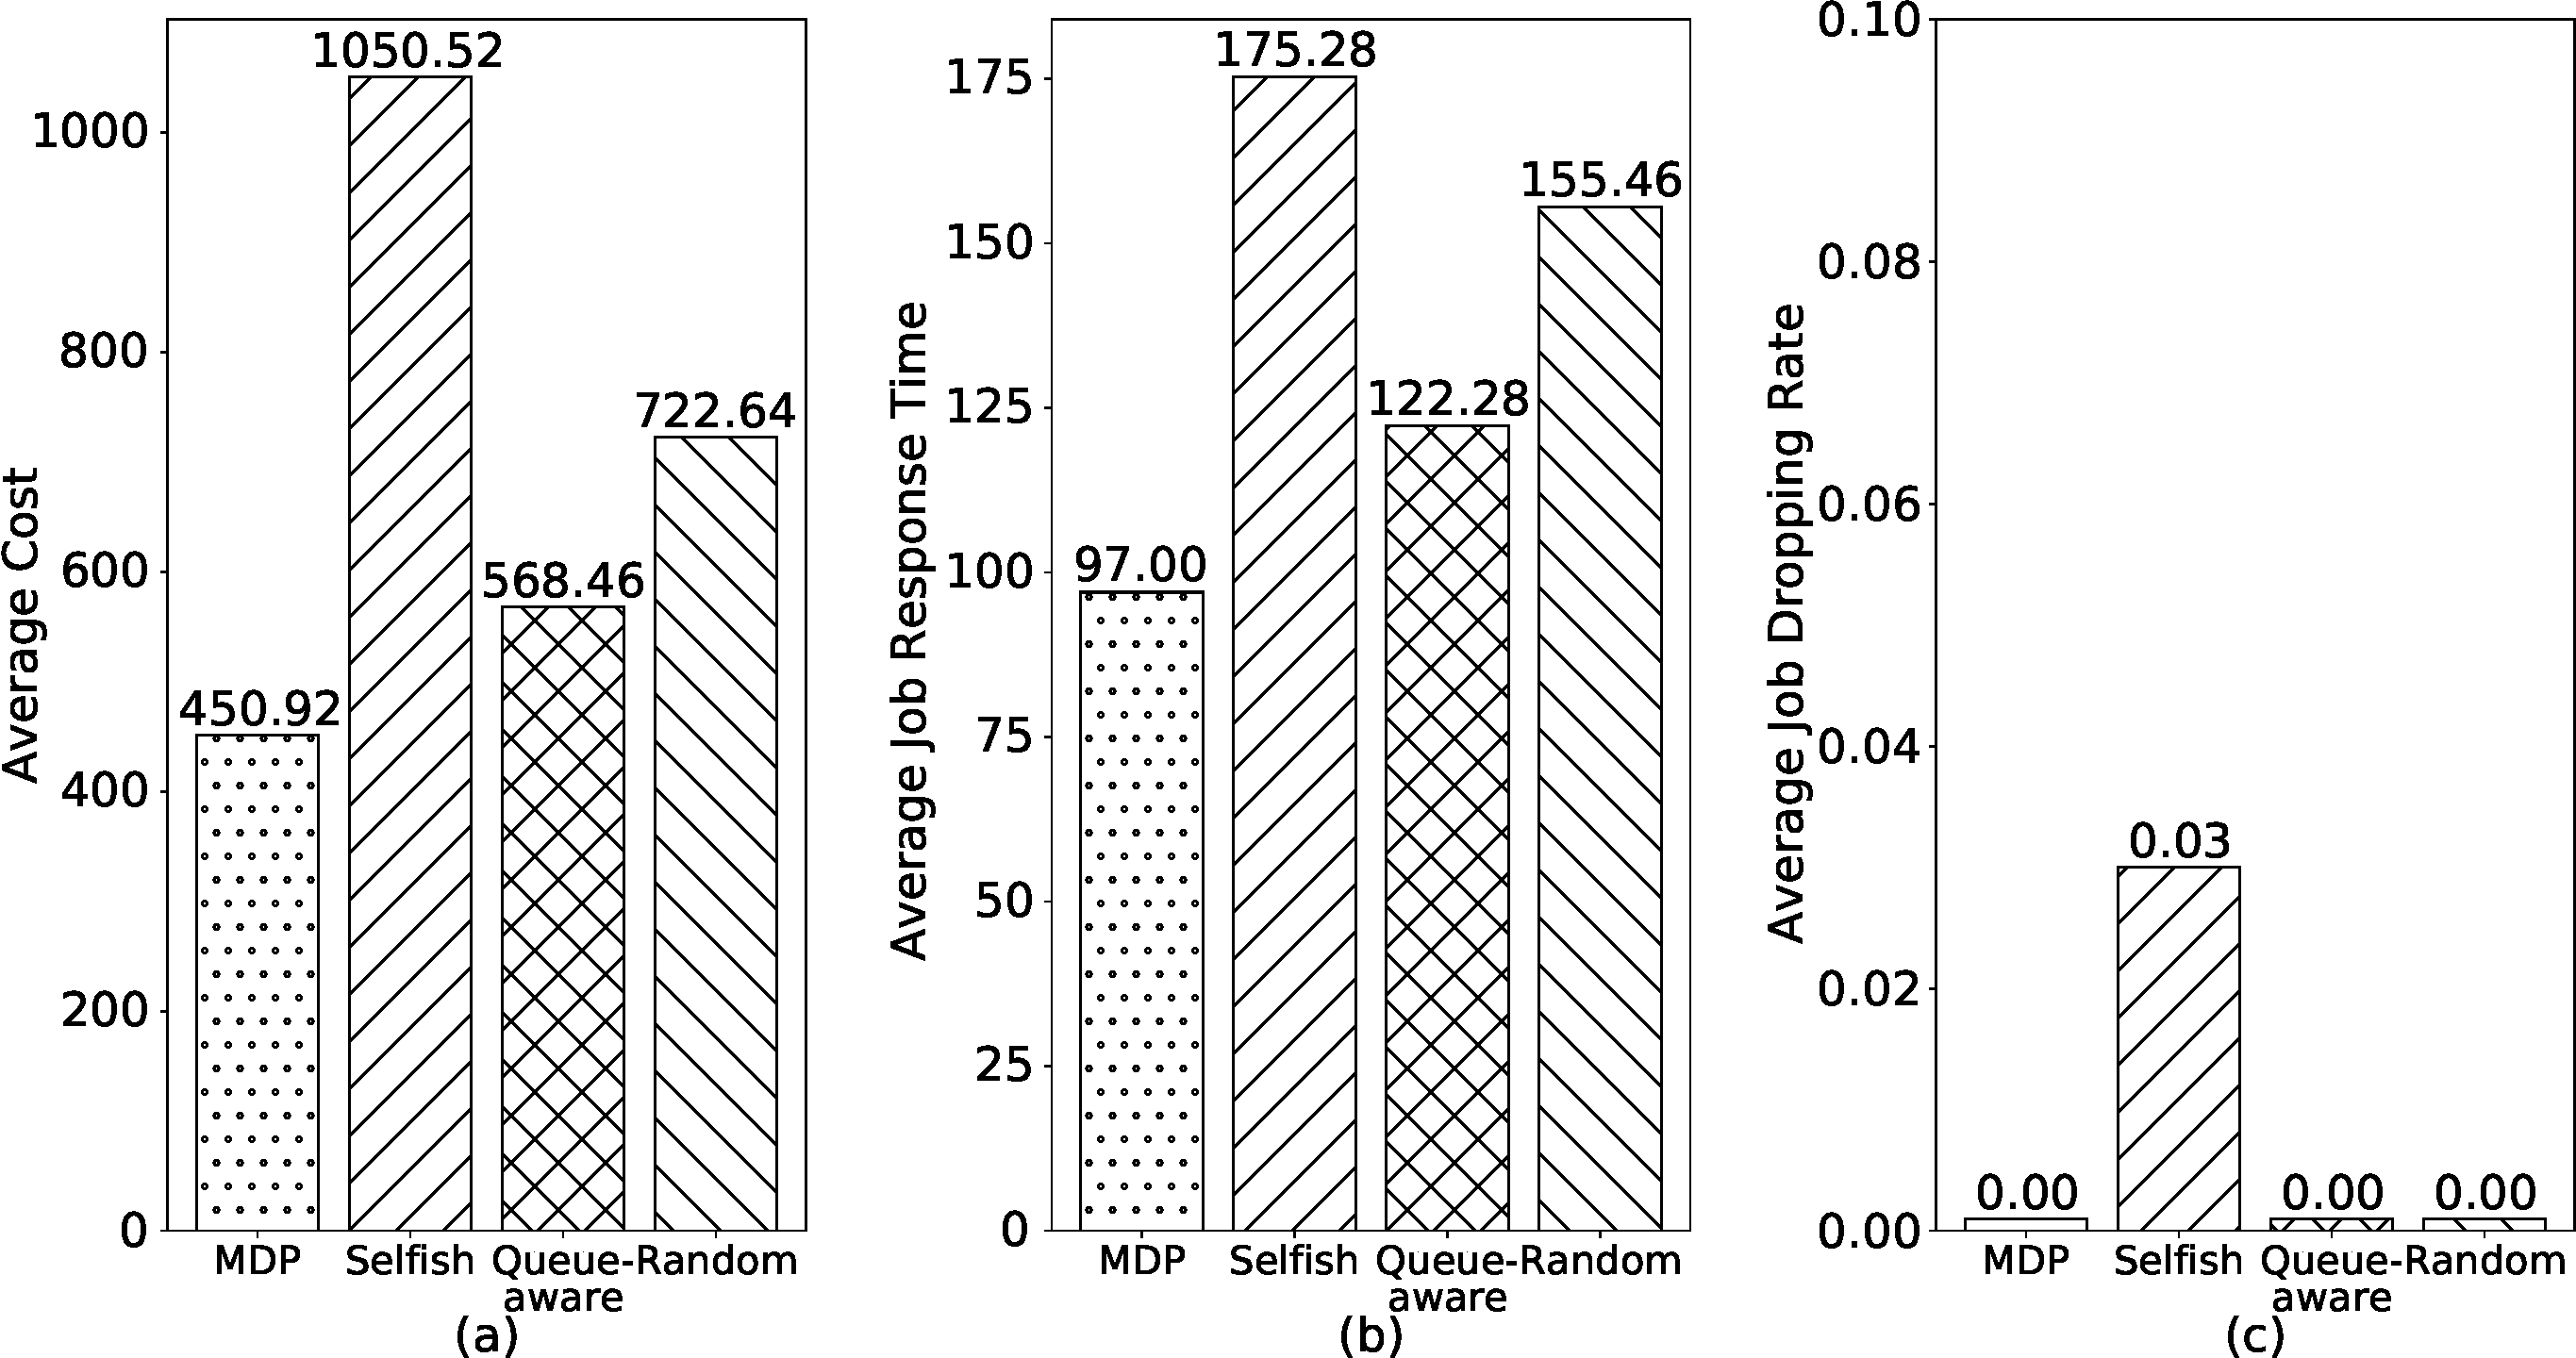
\includegraphics[width=1.0\textwidth]{chapter3/the-bar-graph-alt.pdf}               %
    \caption{Illustration of performance metrics comparison with benchmarks.}
    \label{fig:bar_plot}                                                %
\end{figure*}                                                            %
%-----------------------------------------------------------------------%

%NOTE: Benchmark Elaboration
We also propose three heuristic benchmarks to profile the performance of the proposed solution framework {\Dalgname}, which are listed as follows.
\begin{itemize}
    \item \textbf{Random Policy}:
            Randomly choose a dispatching edge server in each time slot; 
    \item \textbf{Selfish Policy}:
            Always choose the edge server with the minimum sum of the expected uploading time and processing time;
    \item \textbf{Queue-aware Policy}:
            Always choose the edge server with the minimum sum of expected uploading time, processing time and queueing time based on the observation of outdated queue status.
\end{itemize}
Moreover, we choose the Selfish Policy as the initial dispatching action (Baseline Policy) for our proposed algorithm (Algorithm \ref{alg_1}).

%NOTE: Basic Performance
\subsection{Performance Analysis}
\label{subsec:chapter3-basic}
As illustrated in \figurename~\ref{fig:bar_plot}(a), the proposed policy (MDP Policy) outperforms all the benchmarks in the average system cost.
Moreover, the Queue-aware Policy has better performance than the other benchmarks due to its capability of adapting dispatching action according to the outdated observation of queueing state.
More insights on the performance comparison are provided in \figurename~\ref{fig:bar_plot}(b) and (c).

In the former figure, the average job response times, measuring the average number of broadcast intervals from job's arrival at one AP to the completeness of computation at one edge server, are compared.
It can be observed that the proposed policy still outperforms all the benchmarks.
In \figurename~\ref{fig:bar_plot}(c), the job dropping rates, measuring the ratio of jobs dropped by edge servers due to queue overflow, are also compared.
{In} summary, the proposed policy outperforms {the} other three benchmarks with the minimum average cost and job response time.
{Moreover, there {are} no dropping jobs incurred compared with the Selfish policy, which is the initial baseline policy for our proposed algorithm.}

Finally, a realization of job dispatching is illustrated in \figurename~\ref{fig:general_timeline}, where the number of jobs in the system is plot versus the index of broadcast interval.
It can be observed that the proposed policy {manages} to keep the number of jobs {at a} lower level, compared with the other benchmarks.
This demonstrates its high dispatching efficiency.

In \figurename~\ref{fig:semi-bound}, the simulation result demonstrates the vanishing gap between the semi-analytical cost upper bound $W^{(T)}_{\hat{\Baseline}}(\Stat)$ and the actual average performance of the proposed policy for different $T$.
It shows that the proposed policy $\tilde{\Policy}$ is bounded and the performance gap $e(T)$ decreases monotonically when $T$ increases, leading to a trade-off between evaluation accuracy and computation complexity.

%-----------------------------------------------------------------------------------------------%
\begin{figure*}[ht!]                                                                             %
    \centering                                                                                  %
    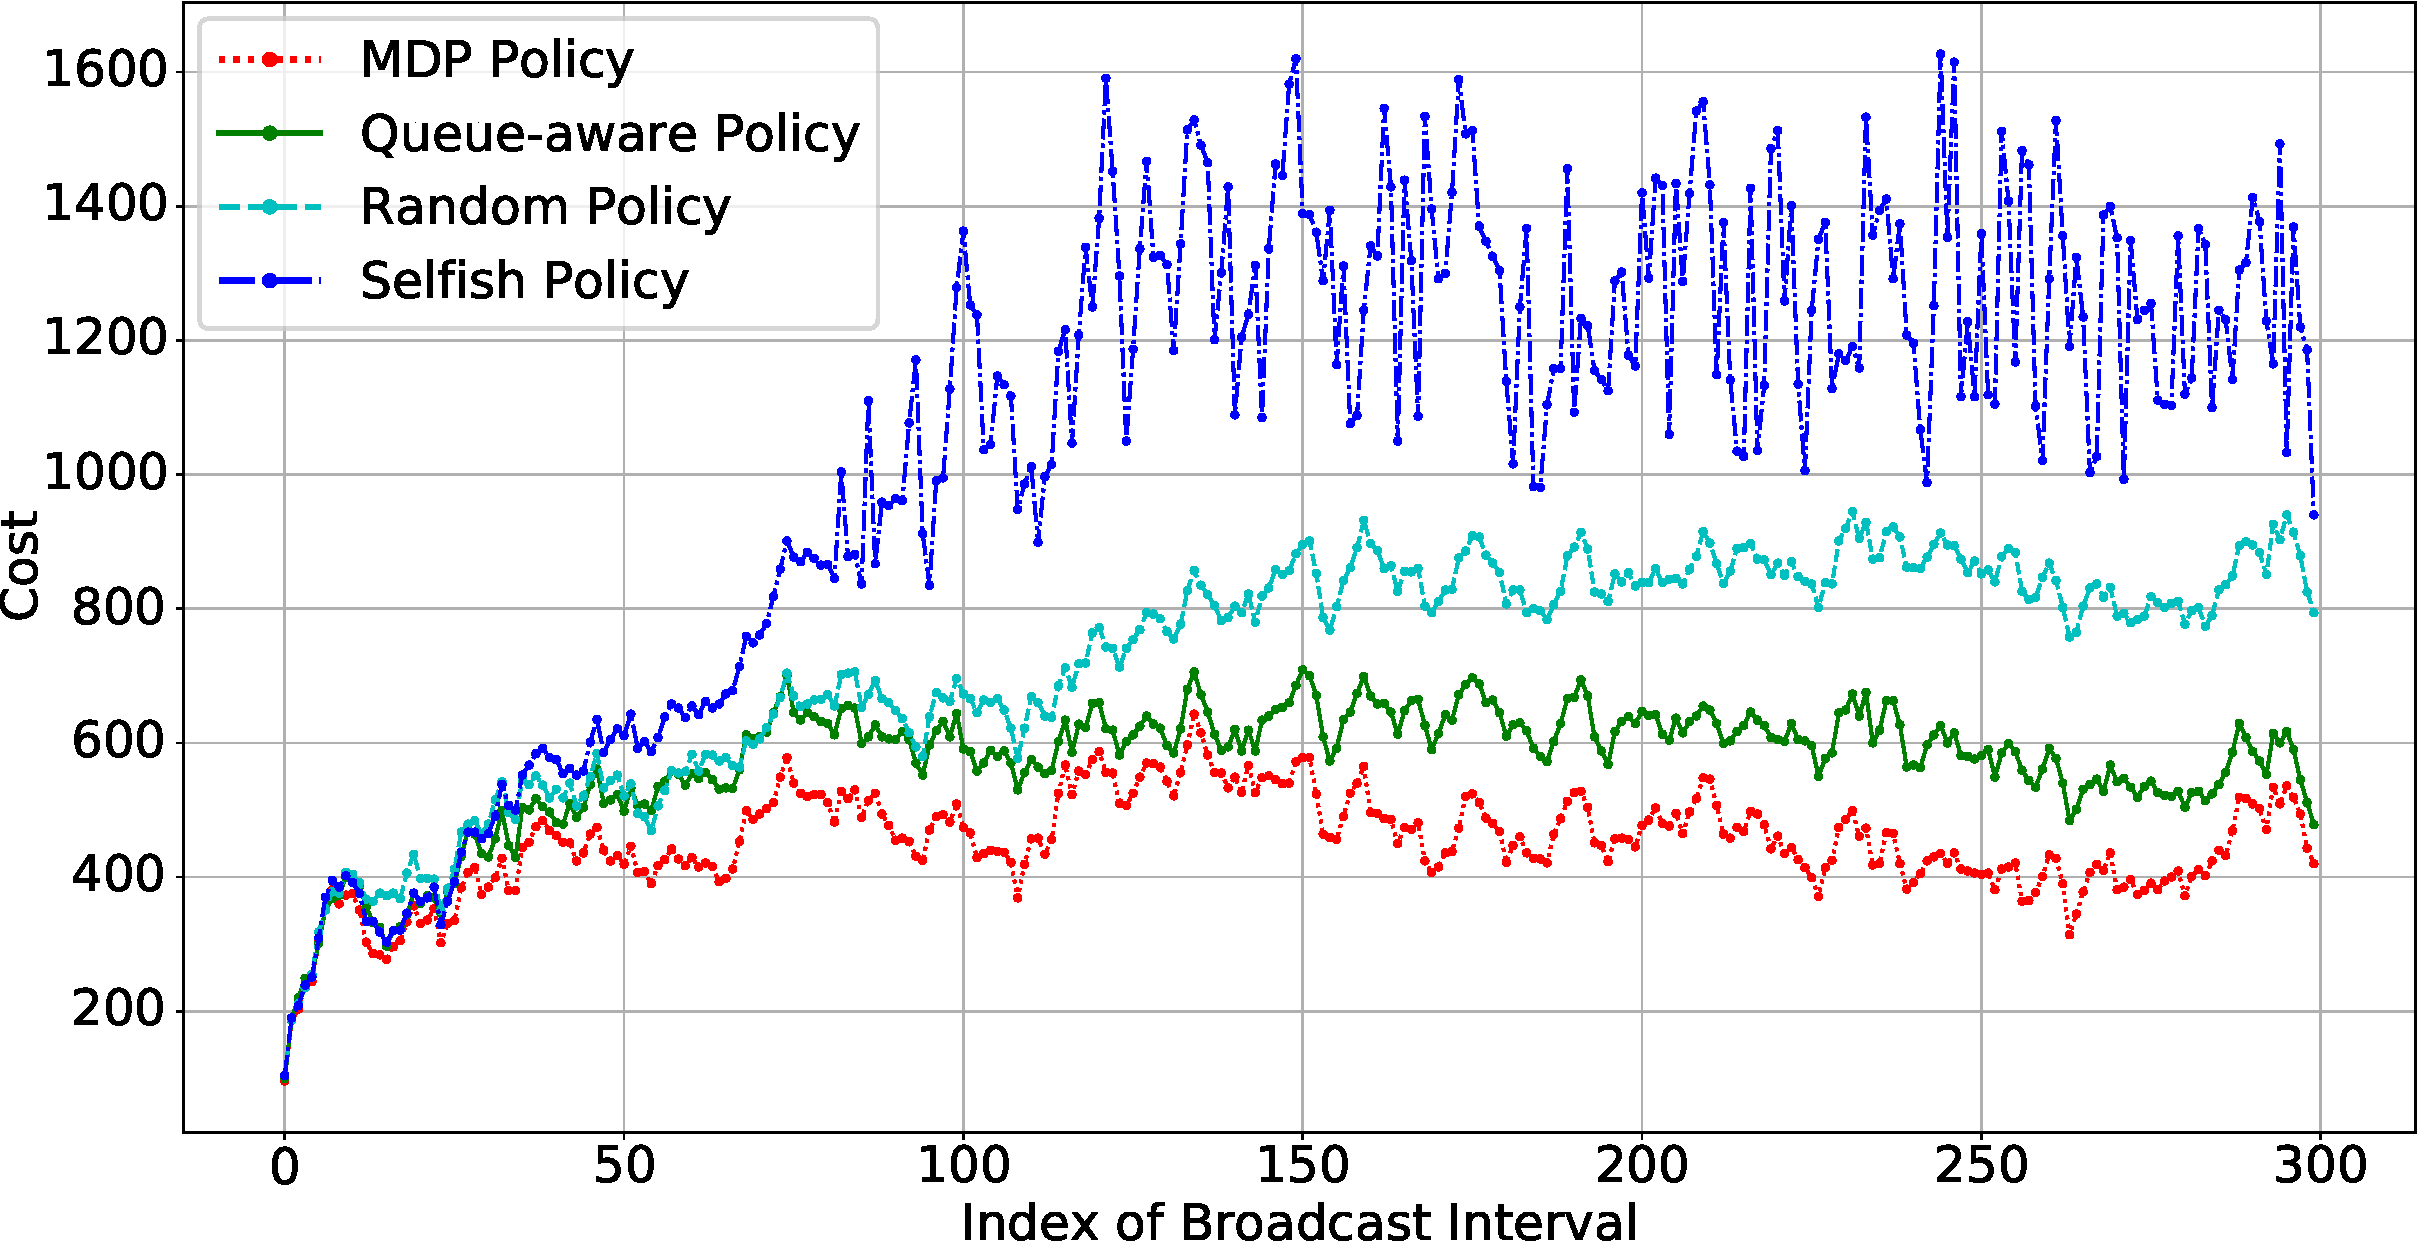
\includegraphics[width=1.0\textwidth]{chapter3/the-cost-timeline-alt.pdf}                     %
    \caption{Illustration of cost versus index of broadcast interval.}
    \label{fig:general_timeline}                                                                %
\end{figure*}                                                                                    %
%-----------------------------------------------------------------------------------------------%

%-----------------------------------------------------------------------------------------------%
\begin{figure*}[ht!]                                                                             %
    \centering                                                                                  %
    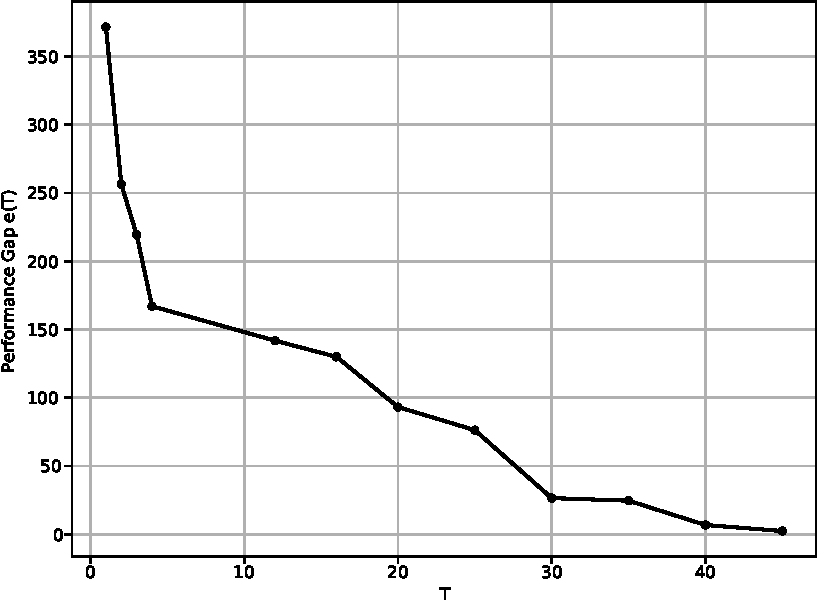
\includegraphics[width=1.0\textwidth]{chapter3/the-semi-bound-analysis.pdf}                     %
    \caption{Illustration of performance gap between $W^{(T)}_{\hat{\Baseline}}(\Stat)$ and $W_{\tilde{\Policy}}(\Stat)$ versus the stage number of numerical evaluation T.}
    \label{fig:semi-bound}                                                                %
\end{figure*}                                                                                    %
%-----------------------------------------------------------------------------------------------%

%NOTE: Reinforcement Learning Analysis
\subsection{Convergence Analysis}
\label{subsec:chapter3-converge}
The convergence property of the proposed reinforcement learning algorithm is illustrated in \figurename~\ref{fig:rl_plot}.
It can be observed that the learning procedures for all the three statistical parameters converge after $80$ broadcast intervals.
On the other hand, the number of observations required for the convergence of conventional reinforcement learning algorithms is usually larger for enormous system and action space.
This demonstrates the efficiency of the proposed reinforcement learning algorithm, which benefits from the derived expression {of} the approximate value function.
\begin{figure*}[ht!]
    \centering
    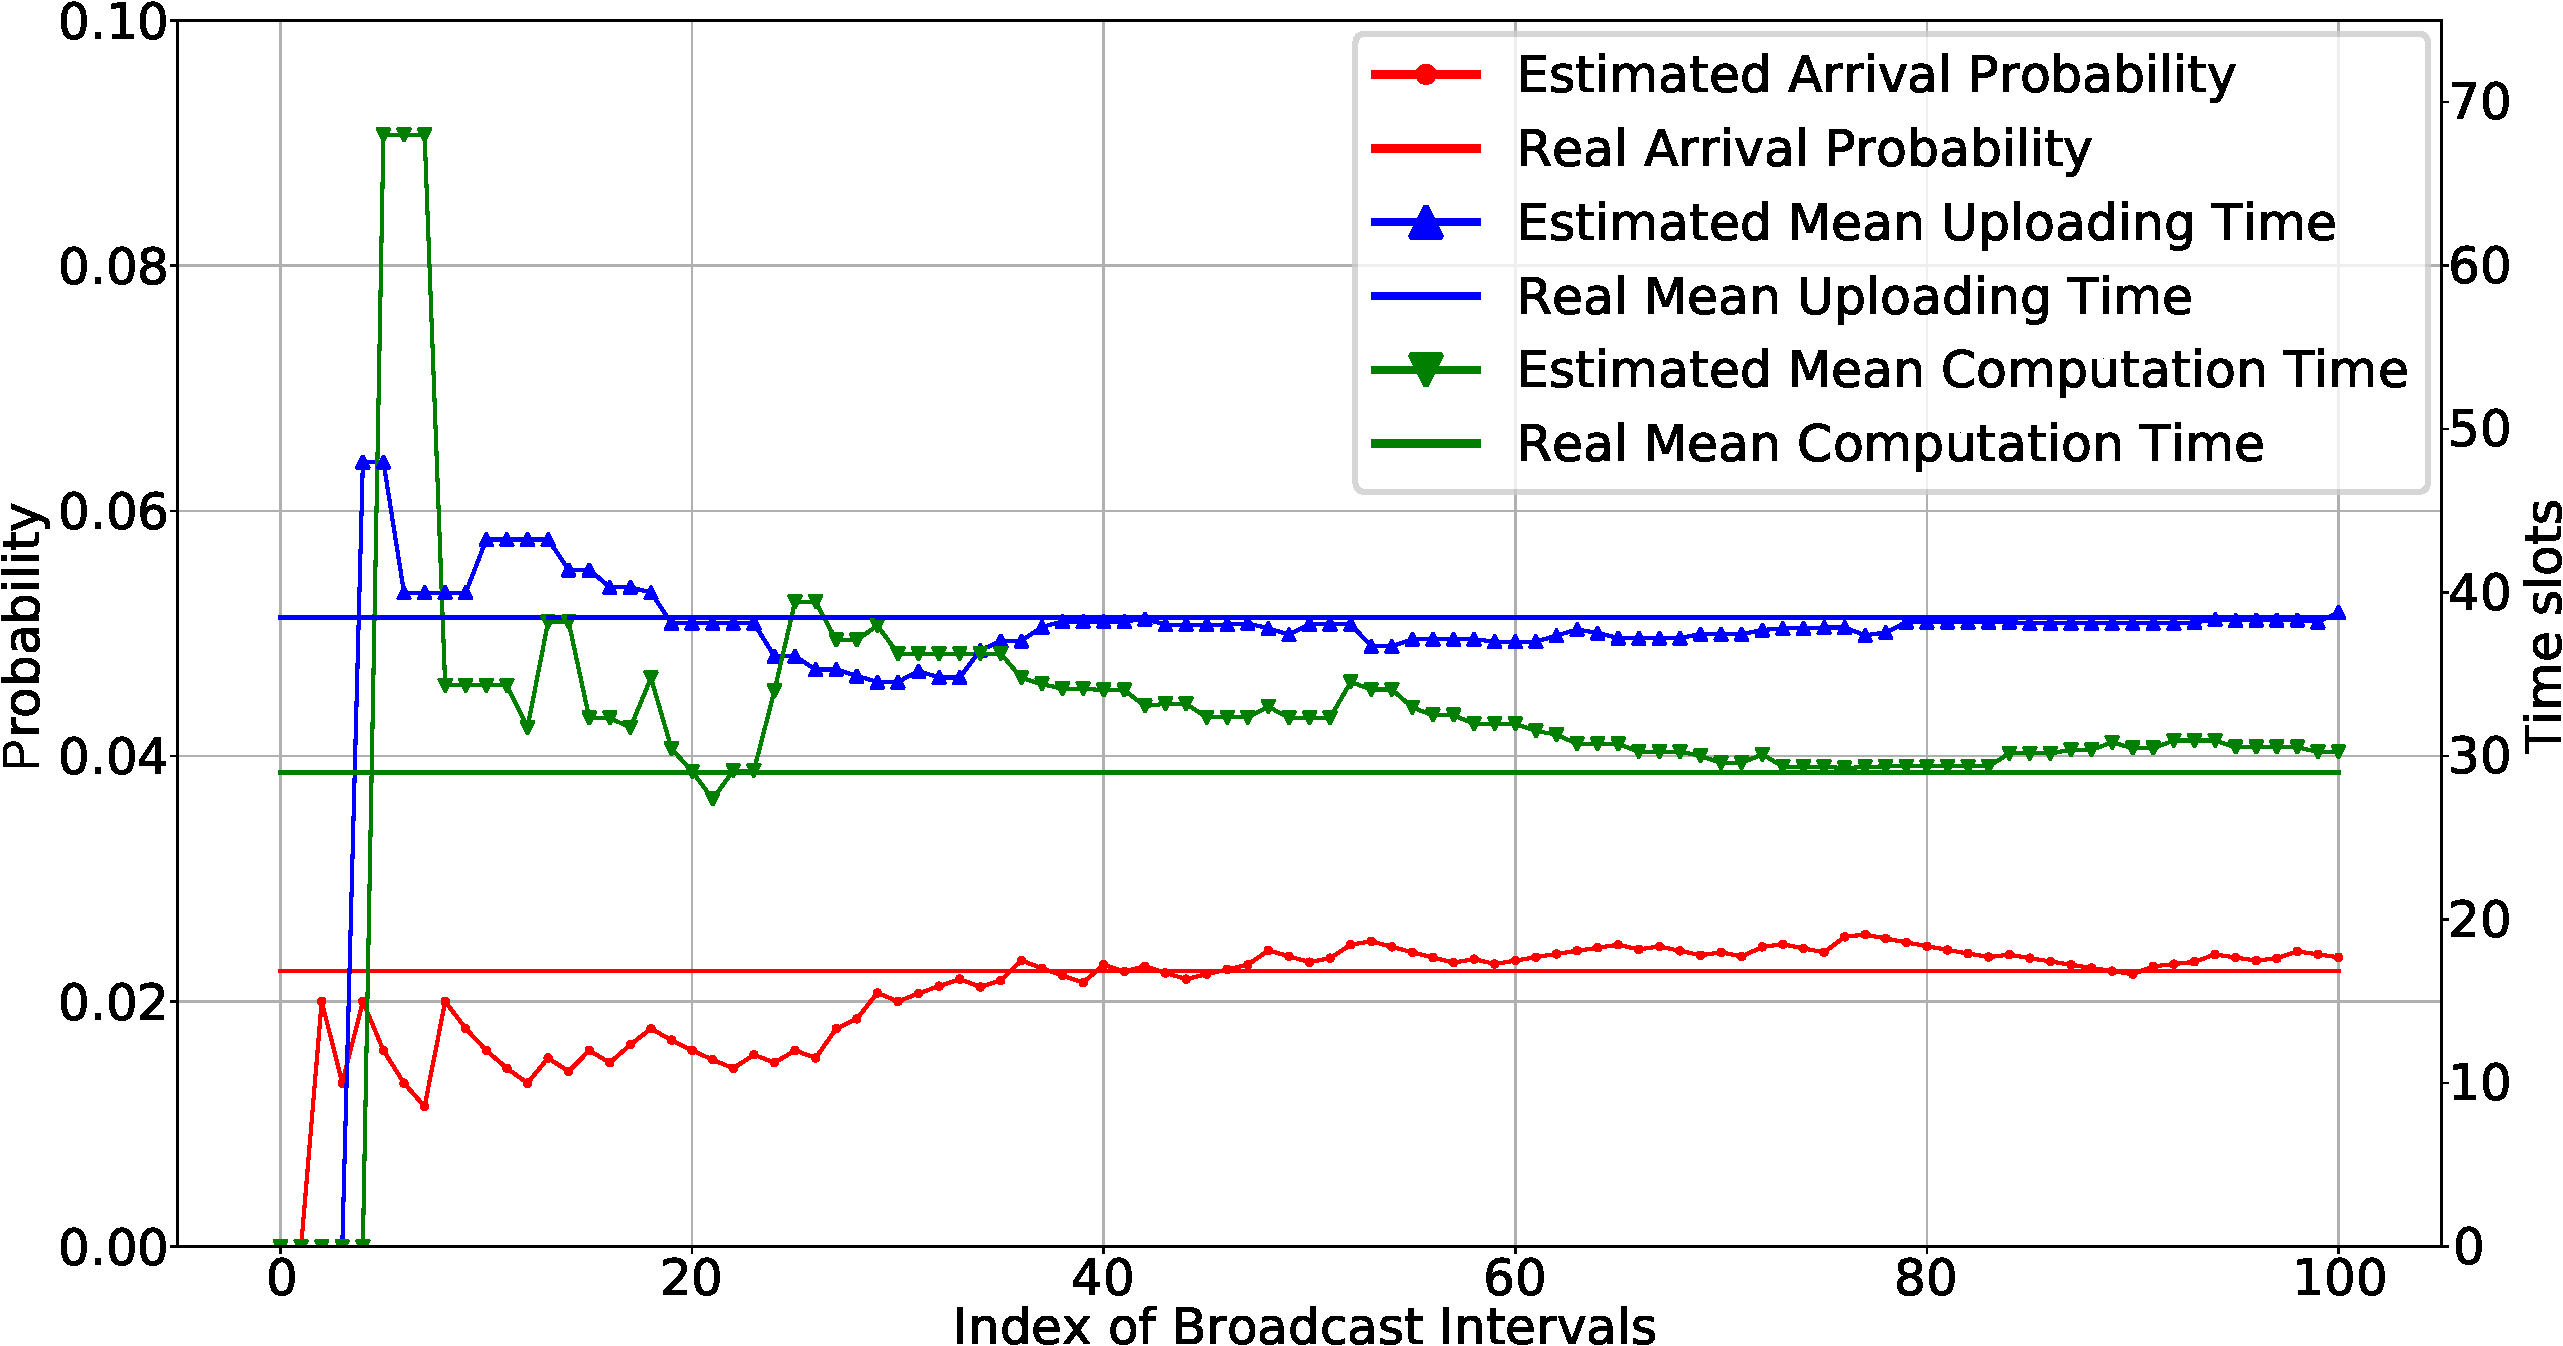
\includegraphics[width=1.0\textwidth]{chapter3/the-rl-fitting.pdf}
    \caption{Illustration of reinforcement learning algorithm.} 
    \label{fig:rl_plot}
\end{figure*}

\subsection{Sensitivity Study}
\label{subsec:chapter3-advance}
%-----------------------------------------------------------------------------------%
\begin{figure*}[ht!]                                                                %
    \centering                                                                      %
    \begin{minipage}[b]{0.65\textwidth}                                             %
        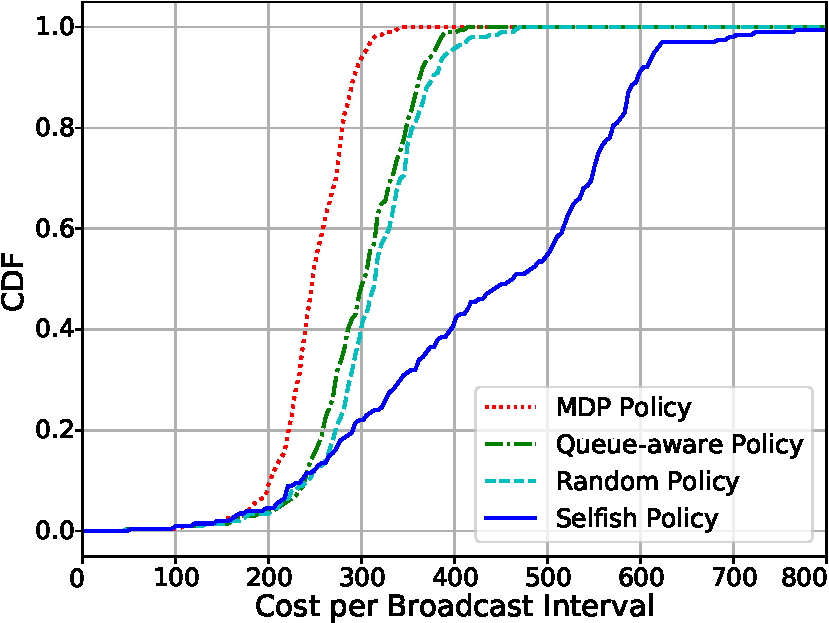
\includegraphics[width=\textwidth]{chapter3/the-delay-small.pdf} \\         %
        (a) Latency = $5$ time slots                                                %
        %\\ % extra filling line                                                    %
    \end{minipage}                                                                  %
    \begin{minipage}[b]{0.65\textwidth}                                             %
        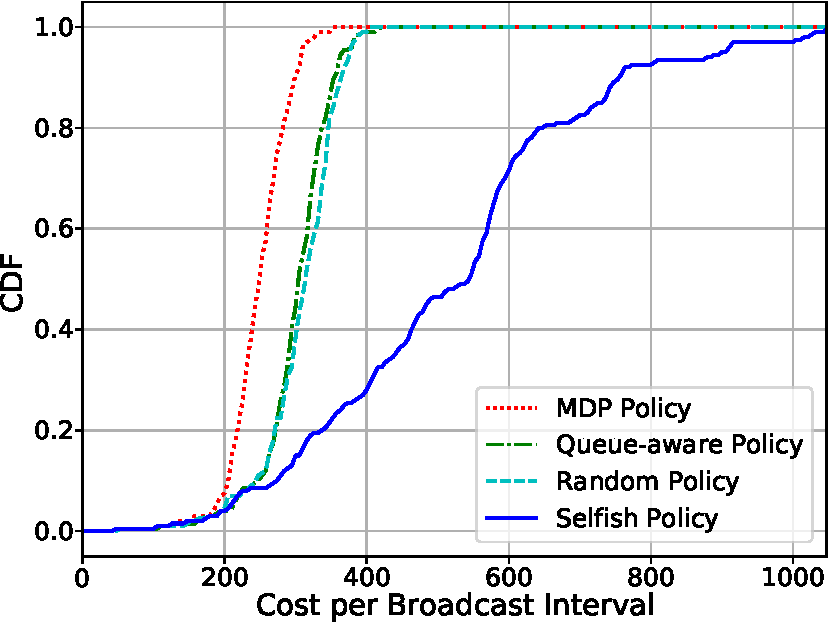
\includegraphics[width=\textwidth]{chapter3/the-delay-medium.pdf} \\        %
        (b) Latency = $12$ time slots                                               %
    \end{minipage}                                                                  %
    \begin{minipage}[b]{0.65\textwidth}                                             %
        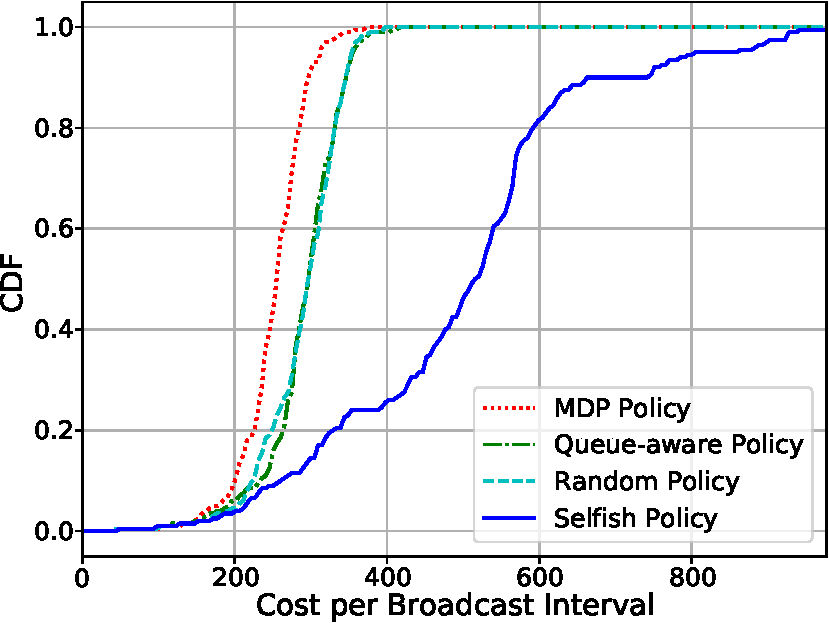
\includegraphics[width=\textwidth]{chapter3/the-delay-large.pdf} \\         %
        (c) Latency = $25$ time slots                                               %
    \end{minipage}                                                                  %
    \caption{Algorithm Robustness versus various signaling latency.}                %
    \label{fig:ss_signal}                                                           %
\end{figure*}                                                                       %
%-----------------------------------------------------------------------------------%


%-------------------------------------------------------------------%
\begin{figure*}[hbt]                                                 %
    \centering                                                      %
    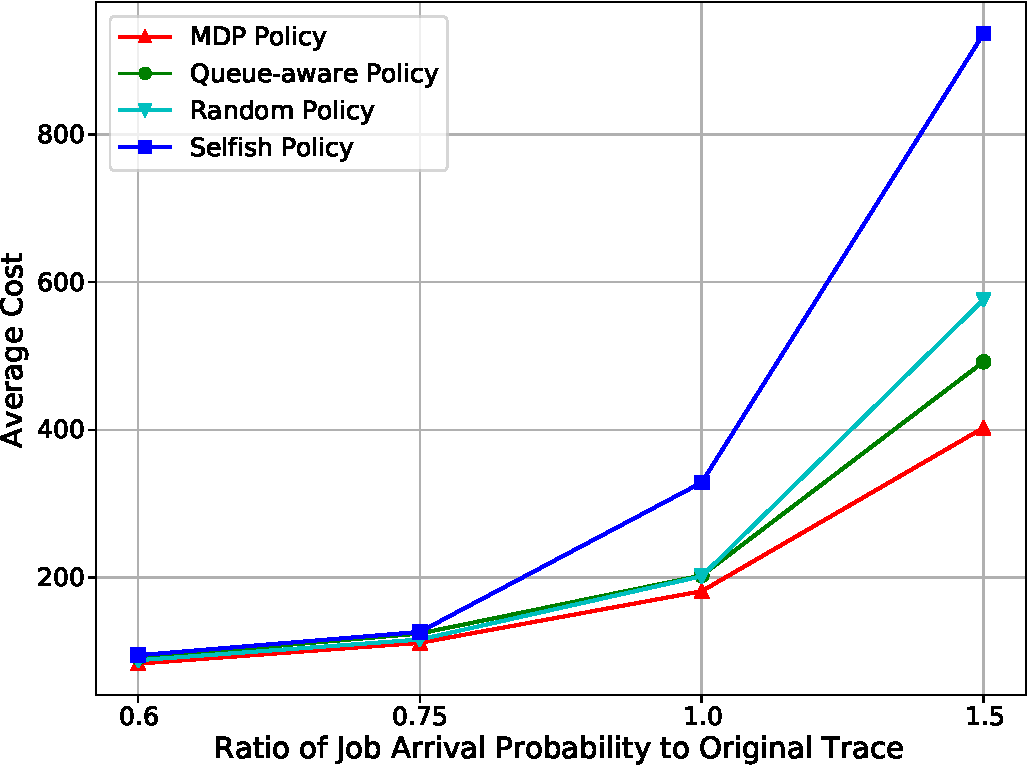
\includegraphics[width=1.0\textwidth]{chapter3/the-arrival-study.pdf}   %
    \caption{Illustration of average system cost versus job arrival intensity.}
    \label{fig:ss_scale}                                            %
\end{figure*}                                                        %
%-------------------------------------------------------------------%

%-------------------------------------------------------------------%
\begin{figure*}[hbt]                                                 %
    \centering                                                      %
    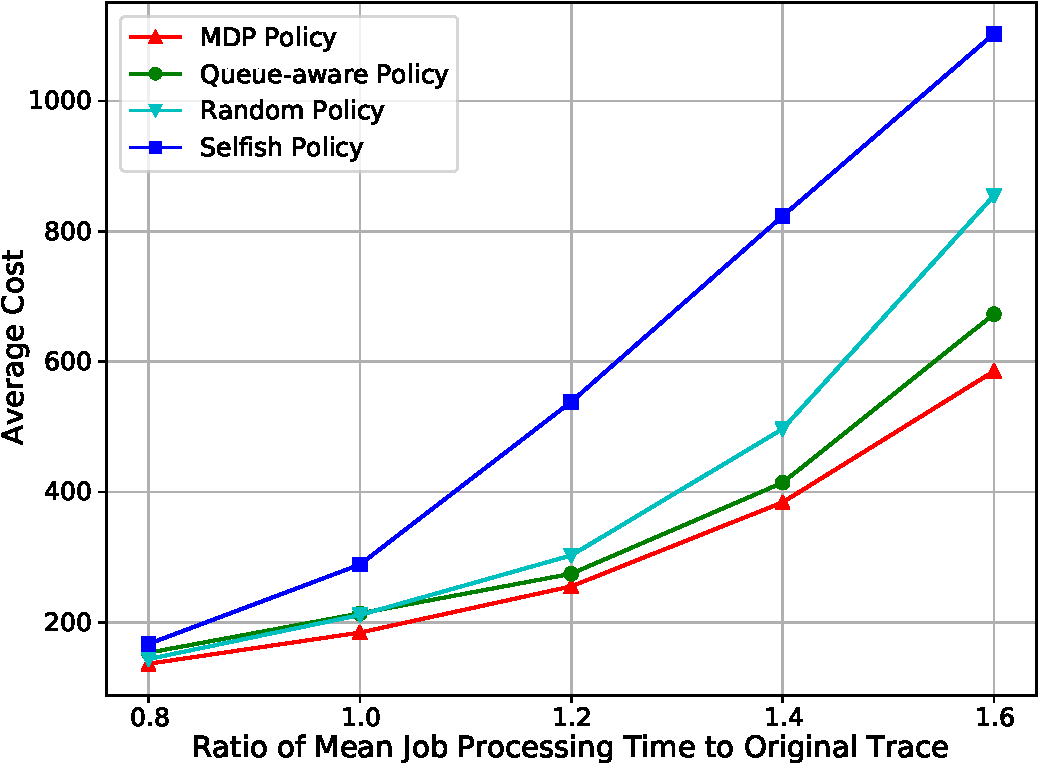
\includegraphics[width=1.0\textwidth]{chapter3/the-proc-study.pdf}      %
    \caption{Illustration of average system cost versus mean processing time.}
    \label{fig:ss_dist}                                             %
\end{figure*}                                                        %
%-------------------------------------------------------------------%

%NOTE: sensitivity study
\noindent\textbf{Signaling Latency.}
The simulation results with different {\brlatency} $\mathcal{D}_{k}$ ($\forall k\in\apSet$) are illustrated in \figurename~\ref{fig:ss_signal}, where the cumulative distribution function (CDF) of the job number in the system is plotted.
Specifically, the {\brlatency} of all the APs is set to $5, 12, 25$ in \figurename~\ref{fig:ss_signal}(a), \figurename~\ref{fig:ss_signal}(b), \figurename~\ref{fig:ss_signal}(c), respectively.
It can be observed from \figurename~\ref{fig:ss_signal}(a) to \figurename~\ref{fig:ss_signal}(c) that, with the increasing of {\brlatency}, the performance of Queue-aware Policy becomes worse.
The Queue-aware policy slightly outperforms the Random Policy in \figurename~\ref{fig:ss_signal}(a) with smaller {\brlatency} (achieving a smaller number of jobs in the system), and becomes worse in \figurename~\ref{fig:ss_signal}(c) with large {\brlatency}.
This demonstrates that the Queue-aware Policy is sensitive to the {\brlatency}.
In all the figures, the proposed policy outperforms all the benchmarks, which demonstrates its robustness versus signaling latency.

\noindent\textbf{Job Arrival Probability.}
We carry out the sensitivity study of job arrival probability by scaling the interval of jobs arriving in Google cluster traces.
The average system cost versus the number of APs is illustrated in \figurename~\ref{fig:ss_scale}.
With the {increase} of job arrival probability, the average system cost increases in all the benchmarks and our proposed policy.
It can be observed that our policy performs the best.
Moreover, the performance gain becomes significant when the computation load is heavy.
This demonstrates the dispatching efficiency of the proposed policy with heavy load.
The gain is negligible for light load, where the computation capability is sufficient and dispatcher optimization may not be necessary.

\noindent\textbf{Mean Processing Time.}
The simulation results with different mean processing time $\set{c_{m,j}|\forall m\in\esSet,j\in\jSpace}$ are illustrated in \figurename~\ref{fig:ss_dist}, where the average processing time from Google cluster traces is scaled by a factor from $0.8$ to $1.6$ respectively.
in our computation model assumption.
Generally speaking, with the increasing average processing time, the average system cost increases in all the benchmarks and our proposed policy.
The simulation results are consistent with that in \figurename~\ref{fig:ss_scale}.
It can be observed that the proposed policy has better performance than the benchmarks.
Moreover, the performance gain becomes significant when the computation time is long.

%=================================================================================================%
%=================================================================================================%

\section{Summary}
\label{sec:chapter3-conclusion}
In this chapter, we consider a distributed and asynchronous job dispatching design in an edge computing network residing in a MAN with multiple APs and edge servers.
The APs and edge servers periodically broadcast their local state information to facilitate distributed dispatcher design.
Due to random transmission latency, the system information observed at different dispatchers are asynchronous.
We also consider a practical scenario that not all the state information can be observed by each AP.
Hence, the distributed optimization of job dispatching strategies at all the APs is formulated as a POMDP, whose minimization objective is a discount measurement of job delivery and computation time.
We propose a novel low-complexity distributed solution framework, called {\Dalgname}, based on analytical approximation of value function and one-step policy iteration, where the complicated POMDP solution or value iteration is avoided. Both the analytical and semi-analytical performance lower bounds are derived for the approximate MDP solution.
Furthermore, to handle a general scenario where the statistics of signaling latency, uploading latency and computation time are unknown in advance, an efficient online learning approach is proposed.
The simulation results show that the proposed solution framework outperforms various heuristic baselines.
